\documentclass{mcmthesis}
\mcmsetup{CTeX = false, 
  tcn = 2622395, problem = A,
  sheet = true, titleinsheet = true, keywordsinsheet = true,
  titlepage = false, abstract = true}

\usepackage{palatino}
\usepackage{amsmath}
\usepackage{amssymb}
\usepackage{graphicx}
\usepackage{subfigure}
\usepackage{algorithm}
\usepackage{algpseudocode}
\usepackage{booktabs} % For professional tables
\usepackage{float}
\usepackage{indentfirst} % Indent first paragraph
\usepackage{array}
\usepackage{geometry}
\usepackage{multirow} % For complex tables
\usepackage{tabularx} % For auto-width tables
\usepackage{url} % For formatting URLs

% Define standardized math commands for consistency
\newcommand{\SOC}{\text{SOC}}
\newcommand{\Vterm}{V_{terminal}}
\newcommand{\Vocv}{V_{OCV}}
\newcommand{\Pload}{P_{load}}
\newcommand{\Vp}{V_{p}}
\newcommand{\Qcap}{Q_{capacity}}
\newcommand{\Qmax}{Q_{max}}
% New commands for thermal model
\newcommand{\Rtotal}{R_{total}}
\newcommand{\Tref}{T_{ref}}

\title{The Pulse of Power: A Multi-Physics Coupled Thevenin Model for Smartphone Battery Dynamics}

\begin{document}

% =========================================================
% Summary Sheet
% =========================================================
\begin{abstract}
\hspace{2em}Smartphones have become an integral part of daily life, yet their battery performance remains notoriously unpredictable. To provide practical usage recommendations, we establish a continuous-time mathematical model that integrates the physicochemical principles of lithium-ion batteries with auxiliary datasets.

For \textbf{Task 1}, we propose a \textbf{"Component Power-Electrochemical State Coupled Model."} We first employ a continuous-time 1st-order \textbf{Thevenin Equivalent Circuit Model (ECM)} to represent the battery's internal state, incorporating the \textbf{Arrhenius relation} to simultaneously correct for the non-linear effects of temperature on internal resistance and available capacity. Building on this, we expand the framework with a Multi-Factor Power Model, deviding the total load into four physical components: Screen, CPU, Network, and Background. We then utilize \textbf{NNLS} on public datasets to identify parameters for both the battery dynamics and power components, laying the foundation for prediction.

For \textbf{Task 2}, to predict TTE under varying initial states and scenarios, we integrate the load model, Thevenin equations, and thermal corrections into a \textbf{Closed-Loop Predictor}. The iterative process employs \textbf{FFRLS} for online parameter updates and an \textbf{AUKF} for state estimation (SOC/Terminal Voltage), resolving current via the power-voltage analytical constraint. We quantify uncertainty using \textbf{Bootstrap resampling}, providing 90\% confidence intervals. Results demonstrate that low-temperature, high-load conditions precipitate the fastest depletion.

For \textbf{Task 3}, to identify the drivers of endurance variability, we construct a \textbf{Morris Global Sensitivity Analysis} combined with \textbf{Bayesian Hypothesis Testing} to statistically validate sensitivity stability. The results reveal that \textbf{Background power consumption} exhibits the strongest and most stable sensitivity.

Finally, in \textbf{Task 4}, we establish a Priority Scoring Model evaluating factors based on Impact Strength, Energy-Saving Potential, and Implementation Cost. Using the \textbf{CRITIC method} for objective weighting, we calculate comprehensive scores to rank power-saving strategies. "Background Management" ranks highest, followed by "Screen Dimming." Additionally, we develop a Battery Aging Model, utilizing parametric curves to illustrate the impact of Calendar Aging and Cycle Aging on the State of Health (SOH).

Synthesizing these findings, we recommend prioritizing background task reduction to extend runtime and adopting specific charging habits to maintain battery health. We hope this study provides actionable insights for smartphone users worldwide.

\end{abstract}

\begin{keywords}
Thevenin ECM; Arrhenius; NNLS; FFRLS-AUKF; Bootstrap; Morris; CRITIC
\end{keywords}

\maketitle

% =========================================================
% Table of Contents (Optimized for One Page)
% =========================================================
\newpage
\begingroup
\setlength{\parskip}{-2pt} % Compact TOC to fit one page
\tableofcontents
\endgroup
\newpage

% =========================================================
% 1. Introduction
% =========================================================
\section{Introduction}

\subsection{Problem Background}
Smartphones have evolved from simple communication tools into powerful computing hubs. However, the energy density of Lithium-ion batteries has not kept pace with the exponential growth in hardware power consumption. Users frequently face "battery anxiety" due to nonlinear drain behaviors. This unpredictability stems from the complex interplay between component power draw and the battery's electrochemical response, which is highly sensitive to environmental factors like temperature \cite{bressan2025}. Accurately modeling this dynamic system is crucial for predicting Time-to-Empty (TTE).

\begin{figure}[H]
    \centering
    \includegraphics[width=0.8\textwidth]{figures/introduction.png}
    \caption{\textbf{Illustration of Smartphone Battery Dynamics.} This diagram visualizes the core problem: balancing user demands (screen, apps) against physical constraints (battery chemistry, temperature) to optimize runtime.}
    \label{fig:intro_concept}
\end{figure}


\subsection{Restatement of the Problem}

The unpredictability of smartphone battery life stems from a disconnect between user perception and the actual mechanisms of energy consumption. While often attributed simply to "heavy use," the underlying phenomenon involves complex, non-linear interactions between hardware power demands and electrochemical dynamics.

This study aims to construct a mathematical framework linking user behavior with battery physics to deconstruct this complex system. The core objectives are as follows:

\begin{itemize}
    \item \textbf{Constructing a Physics-Driven Model:} A continuous-time model is established to quantify the power consumption of key components—such as screen brightness, processor load, and background tasks—integrated with battery state equations accounting for thermal effects. Parameters are grounded in physical principles and validated through data, rather than relying solely on statistical regression.
    
    \item \textbf{Dynamic Prediction and Attribution:} The model is utilized to simulate TTE across various scenarios, elucidating the mechanisms accelerating depletion under specific conditions, such as low temperatures or high loads. Additionally, uncertainty within predictions is quantified to reflect real-world variability.
    
    \item \textbf{Identifying Key Drivers:} Sensitivity analysis is conducted to isolate the dominant variables affecting battery endurance. By perturbing model inputs—such as ambient temperature or background activity—the core factors influencing battery longevity are determined.
    
    \item \textbf{Providing Optimization Strategies:} Mathematical analyses are translated into practical recommendations, offering a basis for end-users to optimize usage habits and for operating systems to enhance power management protocols, thereby extending runtime and mitigating aging effects.
\end{itemize}

\subsection{Our Work}
To address these challenges systematically, we developed a comprehensive modeling framework as illustrated in Figure \ref{fig:our_work}.

\begin{figure}[H]
    \centering
    \includegraphics[width=1.0\textwidth]{figures/our_work.png}
    \caption{\textbf{Overview of Our Modeling Framework.} This flowchart outlines the sequential progression from model development (Task 1) to simulation (Task 2), sensitivity analysis (Task 3), and strategic optimization (Task 4), highlighting the data flow and logical interconnections.}
    \label{fig:our_work}
\end{figure}

% =========================================================
% 2. Assumptions and Notations
% =========================================================
\section{Assumptions and Notations}

\subsection{General Assumptions}
To simplify the complex electrochemical processes while retaining model fidelity, we formulate the following assumptions:

\paragraph{Assumption 1: Thermal Uniformity.} While internal resistance varies with temperature, we assume the battery temperature $T(t)$ is uniform throughout the cell volume, adopting a lumped thermal model approach.

\paragraph{Assumption 2: Quasi-Stationary Impedance.} The polarization parameters ($R_p, C_p$) are treated as functions of SOC but are considered constant within a single integration time step ($\Delta t = 1s$).

\paragraph{Assumption 3: Irreversible Discharge.} We neglect chemical side reactions, such as self-discharge, focusing solely on load-driven discharge dynamics.

\paragraph{Assumption 4: Battery Choice.} We assume the smartphone utilizes a typical lithium-ion battery with a nominal capacity of $\Qcap = 4000 \text{ mAh}$.

\paragraph{Assumption 5: Baseline State of Health (SOH).} For the modeling and prediction phases in Tasks 1 through 3, we assume the battery is in a pristine condition (SOH = 100\%), meaning current capacity equals nominal capacity and internal resistance is at its manufacturing baseline. Aging effects are treated separately in Task 4.

\subsection{Notations}
\begin{table}[H]
\centering
\caption{Notations}
\begin{tabular}{clc}
\toprule
Symbol & Description & Unit \\
\midrule
$SOC(t)$ & State of Charge at time $t$ & $0 \sim 1$ \\
$\Vterm(t)$ & Terminal Voltage (Closed Circuit Voltage) & V \\
$I(t)$ & Discharge Current (Positive for discharge) & A \\
$\Pload(t)$ & Total Load Power (Sum of all components) & W \\
$\Vocv$ & Open Circuit Voltage (Function of SOC) & V \\
$\Vp(t)$ & Polarization Voltage across RC pair & V \\
$R_0(T)$ & Ohmic Internal Resistance (Temperature Dependent) & $\Omega$ \\
$\Qcap$ & Nominal Battery Capacity (at Ref. Temp) & mAh \\
$\Qmax(T)$ & Max Available Capacity at Temp $T$ & mAh \\
$\eta$ & DC-DC Converter Efficiency & Dimensionless \\
$TTE$ & Time-to-Empty & Hours \\
\bottomrule
\end{tabular}
\end{table}
% =========================================================
% 3. Task 1: Developing the Continuous-Time Model
% =========================================================
\section{Task 1: Developing the Continuous-Time Model}

To accurately simulate the discharge behavior, we establish a coupled framework. We first define the battery's internal dynamics (Thevenin ECM), then model the external load (Component Power), and finally perform parameter identification to validate the model against data.

% --- FIGURE 1 (Flowchart) ---
\begin{figure}[H]
    \centering
    \includegraphics[width=0.9\textwidth]{figures/task1流程图.png}
    \caption{\textbf{The Logical Framework of the Component-Coupled Model.}}
    \label{fig:framework}
\end{figure}

% ---------------------------------------------------------
% 3.1 Battery Dynamics (ECM)
% ---------------------------------------------------------
\subsection{Battery Dynamics Model (Thevenin ECM)}
We adopt a \textbf{1st-Order Thevenin Equivalent Circuit Model (ECM)}. As shown in Figure \ref{fig:ecm}, this model consists of an ideal voltage source $\Vocv$, a temperature-dependent ohmic resistance $R_0(T)$, and a parallel RC network ($R_p, C_p$) capturing polarization \cite{chen2006}.

\begin{figure}[H]
    \centering
    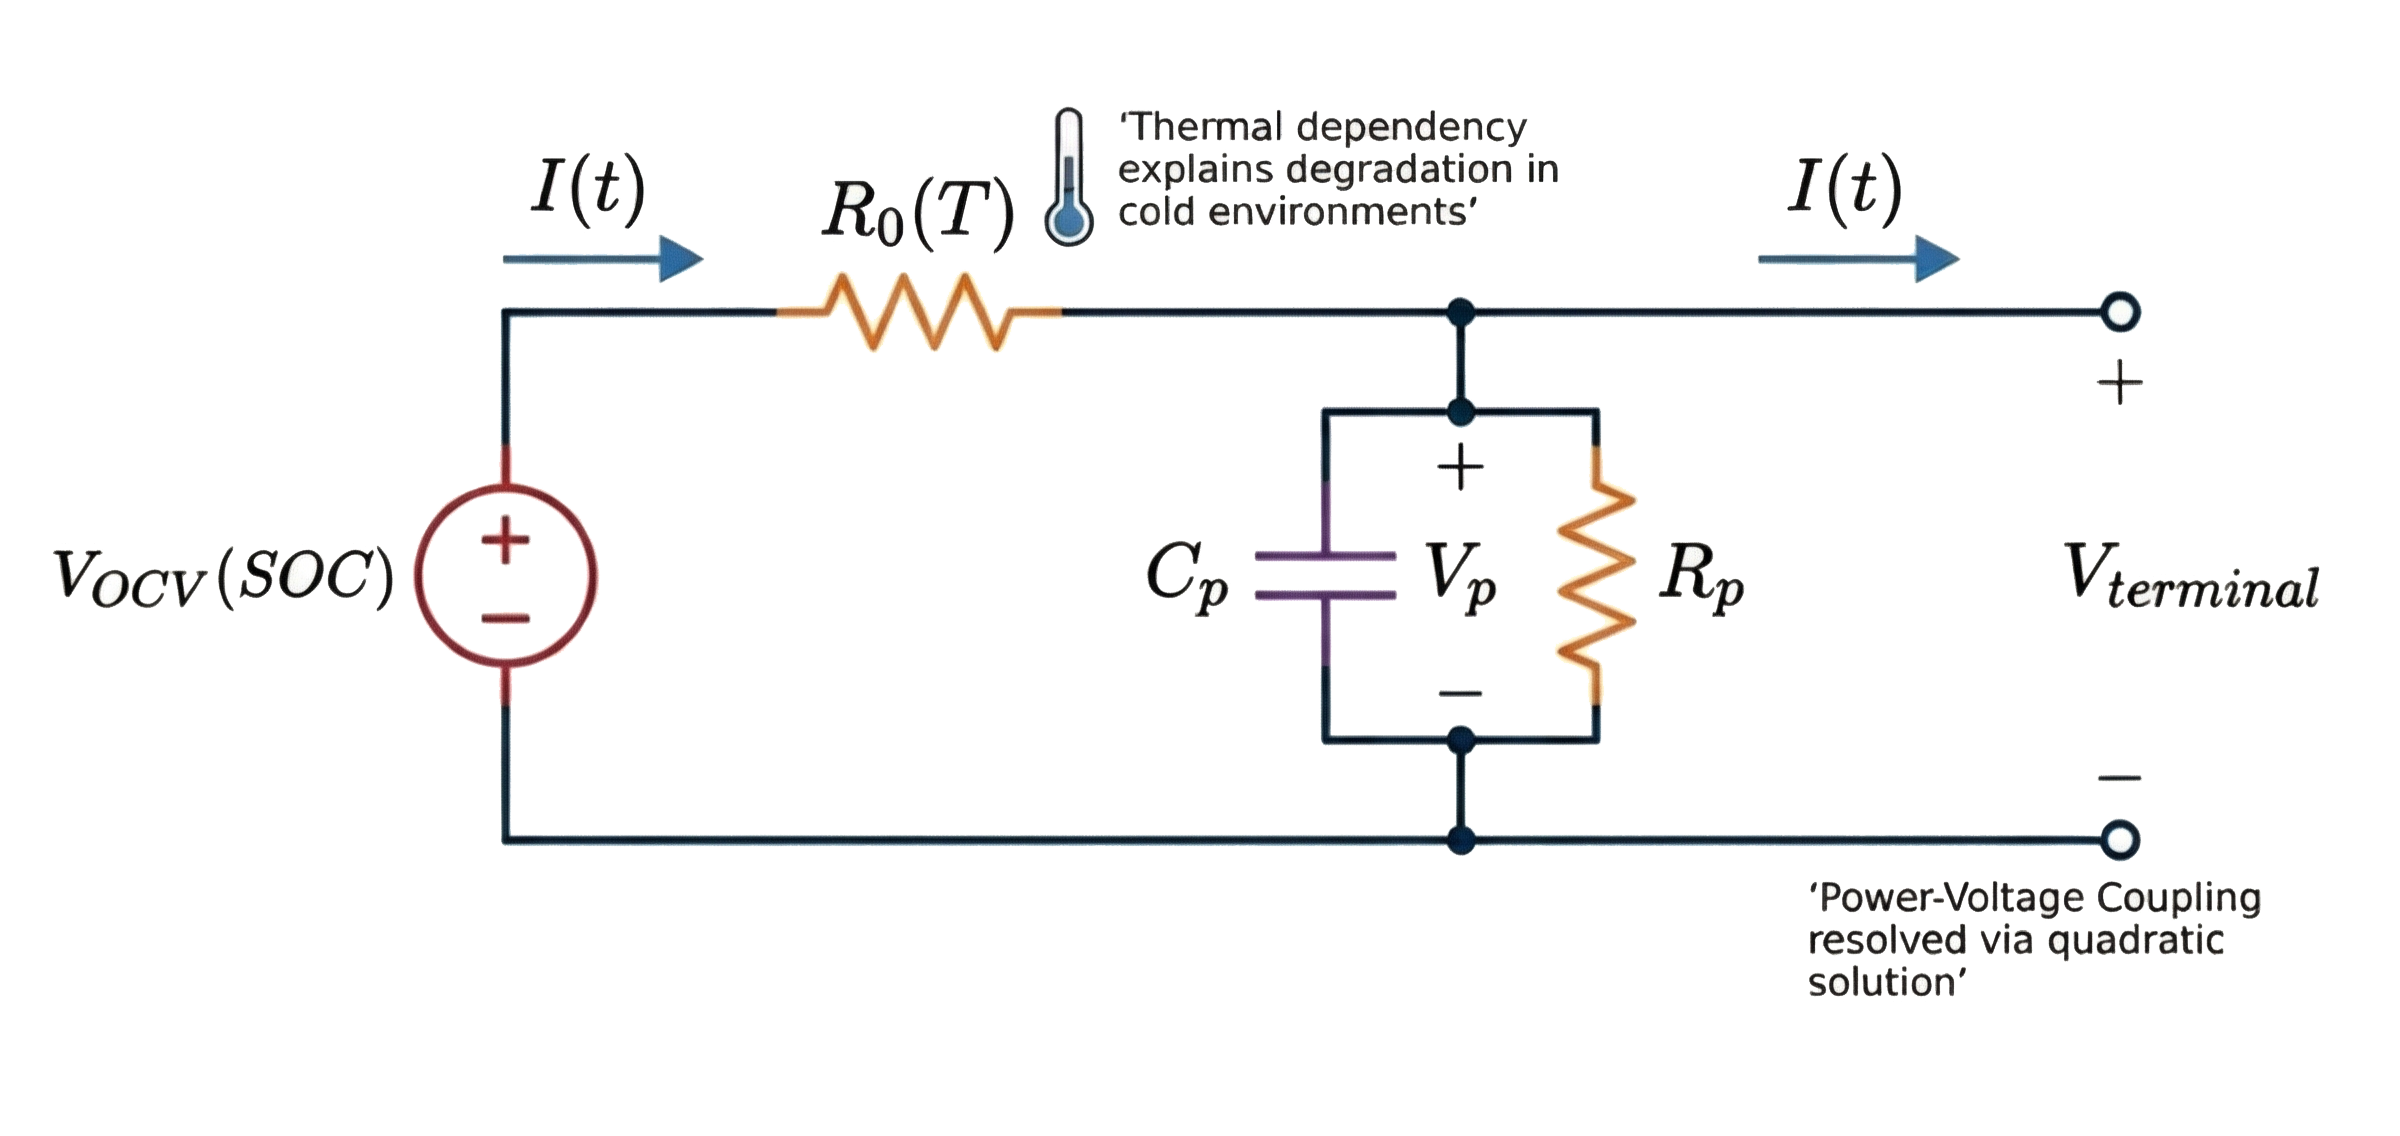
\includegraphics[width=0.7\textwidth]{figures/ECM电路图.png} 
    \caption{\textbf{Schematic of the 1st-Order Thevenin Equivalent Circuit Model.}}
    \label{fig:ecm}
\end{figure}

\subsubsection{State Equations}
\paragraph{SOC Evolution (Coulomb Counting)}
The rate of charge depletion is governed by the current and the temperature-dependent maximum capacity:
\begin{equation} \label{eq:soc_ode}
\frac{d\SOC(t)}{dt} = -\frac{I(t)}{3600 \cdot (\Qmax(T) / 1000)}
\end{equation}

In this equation, we replace the nominal capacity $\Qcap$ with $\Qmax(T)$ to account for the reduced availability of lithium ions at lower temperatures. The constant 3600 converts hours to seconds.

\paragraph{Polarization Dynamics}
The transient response of the battery voltage is modeled as:
\begin{equation} \label{eq:vp_ode}
\frac{d\Vp(t)}{dt} = -\frac{\Vp(t)}{\tau} + \frac{I(t)}{C_p}
\end{equation}

Here, $\tau = R_p C_p$ represents the polarization time constant, characterizing the speed of the voltage recovery or "relaxation effect" observed after load removal.

\subsubsection{Thermal Corrections for Resistance and Capacity}
To accurately model battery behavior under extreme conditions (e.g., cold weather), we apply the \textbf{Arrhenius Law} to modify both internal resistance and available capacity.

\paragraph{Internal Resistance Correction}
Ion mobility decreases exponentially as temperature drops, increasing impedance:
\begin{equation} \label{eq:output}
\Vterm(t) = \Vocv(\SOC(t)) - \Vp(t) - I(t) \cdot R_0(T)
\end{equation}
\begin{equation} \label{eq:arrhenius_R}
R_0(T) = R_{ref} \cdot \exp\left[ \frac{E_a}{R_g} \left( \frac{1}{T(t)} - \frac{1}{\Tref} \right) \right]
\end{equation}

where $R_{ref}$ denotes the resistance at the reference temperature $\Tref$ (typically 298.15 K), $E_a$ is the activation energy characterizing the sensitivity of the electrochemical reaction to temperature, and $R_g$ represents the universal gas constant.

\paragraph{Capacity Correction}
Similarly, the maximum usable capacity $\Qmax(T)$ decreases at lower temperatures due to sluggish electrochemical kinetics. We model this decay using a modified Arrhenius relation:
\begin{equation} \label{eq:arrhenius_C}
\Qmax(T) = \Qcap \cdot \exp\left[ \frac{E_a}{R_g} \left( \frac{1}{\Tref} - \frac{1}{T(t)} \right) \right]
\end{equation}

In this formulation, $\Qmax(T)$ is the maximum available capacity at current temperature $T$ (Ah), $\Qcap$ is the nominal capacity at reference temperature $\Tref$, $E_a$ is the activation energy (typically $15 \sim 30$ kJ/mol), and $R_g$ is the universal gas constant. This dual correction explains why batteries die faster in winter: increased $R_0$ causes premature voltage cutoff, while decreased $\Qmax$ reduces the total energy reservoir.

% ---------------------------------------------------------
% 3.2 Multi-Factor Power Model Expansion
% ---------------------------------------------------------
\subsection{Multi-Factor Power Model Expansion}
The input to our battery model is the total power demand. Based on the principle of physical superposition, the total load power $\Pload(t)$ is the sum of four key factors:
\begin{equation} \label{eq:power_sum}
\Pload(t) = P_{screen}(t) + P_{cpu}(t) + P_{network}(t) + P_{background}(t)
\end{equation}

We analyze the physical characteristics and parameters of each component in detail below.

\paragraph{Screen Power Dynamics}
The screen is often the largest power consumer. We model it using a linear-gamma function relative to brightness:
\begin{equation}
P_{screen}(t) = \beta_0 + \beta_1 \cdot L(t)^\gamma
\end{equation}

Here, $\beta_0$ is the baseline power consumption of the display panel driver circuit (W), $\beta_1$ denotes the luminous efficacy coefficient (W/nit), $L(t)$ represents the normalized screen brightness level ($0 \le L \le 1$), and $\gamma$ is the Gamma correction factor (typically $\approx 2.2$), accounting for the non-linear relationship between human visual perception of brightness and actual light intensity.

\paragraph{Processor Power Dynamics}
Based on CMOS dynamic power theory ($P \propto C V^2 f$), and assuming dynamic voltage frequency scaling (DVFS) where $V \propto f$, the power scales cubically with frequency:
\begin{equation}
P_{cpu}(t) = \sum_{k=1}^{N_{cores}} \alpha_k \cdot f_k(t)^3 \cdot u_k(t)
\end{equation}

where $\alpha_k$ is the effective capacitance coefficient for core $k$, reflecting the specific hardware architecture (e.g., performance cores have larger $\alpha$ than efficiency cores), $f_k(t)$ denotes the operating frequency of core $k$ (Hz), and $u_k(t)$ represents the utilization rate of core $k$ ($0 \le u \le 1$).

\paragraph{Network and Background Power}
Radio Frequency (RF) power consumption is modeled to reflect the exponential cost of maintaining link quality under signal attenuation:
\begin{equation}
P_{network}(t) = c_1 \cdot D_{rate}(t) + c_2 \cdot 10^{\frac{P_{target} - RSSI(t)}{10}}
\end{equation}

where $c_1$ is the energy cost per bit for data transmission (J/bit), $D_{rate}(t)$ denotes the current data throughput (bits/s), $c_2$ is the baseline power for the RF amplifier, $P_{target}$ represents the target reception power level required by the base station (dBm), and $RSSI(t)$ is the Received Signal Strength Indicator (dBm).

Additionally, to account for OS services, sensors, and idle currents, we introduce a background component $P_{background}(t) = k \cdot W_{background}$, where $k$ is a scaling coefficient.

% ---------------------------------------------------------
% 3.3 Power-Voltage Coupling
% ---------------------------------------------------------
\subsection{Power-Voltage Coupling Constraint}
The discharge current $I(t)$ is coupled to the voltage via the constant power constraint of the DC-DC converter:
\begin{equation} \label{eq:coupling}
I(t) = \frac{\Pload(t)}{\Vterm(t) \cdot \eta}
\end{equation}

Substituting Eq. \eqref{eq:coupling} into Eq. \eqref{eq:output} and using the temperature-dependent $R_0(T)$, we obtain a quadratic equation. Solving for the physically valid root gives the analytical solution for the system state at any temperature $T$:
\begin{equation} \label{eq:vterm_solution}
\Vterm(t) = \frac{(\Vocv - \Vp) + \sqrt{(\Vocv - \Vp)^2 - \frac{4 \Pload R_0(T)}{\eta}}}{2}
\end{equation}

% ---------------------------------------------------------
% 3.4 Parameter Identification & Validation
% ---------------------------------------------------------
\subsection{Parameter Identification \& Validation}
We employ a \textbf{Two-Step Fitting Strategy} to estimate parameters. The identification process separates the electrical properties of the battery from the power characteristics of the smartphone hardware.

\subsubsection{Step 1: Electrical Parameters (ECM)}
To ensure the fidelity of the battery dynamics, we reference the verified parameters from the study by Chen \& Rincon-Mora \cite{chen2006}. The typical values for a Lithium-Polymer battery used in our simulation are summarized in Table \ref{tab:ecm_params}. Note that in our notation, the series resistance $R_s$ corresponds to our $R_0$.

\begin{table}[H]
\centering
\caption{Electrical Parameters for the Thevenin ECM \cite{chen2006}}
\label{tab:ecm_params}
\begin{tabular}{lccc}
\toprule
\textbf{Parameter} & \textbf{Symbol} & \textbf{Typical Value} & \textbf{Unit} \\ 
\midrule
Series Resistance & $R_0$ & 0.082 & $\Omega$ \\
Polarization Resistance & $R_p$ & 0.015 & $\Omega$ \\
Polarization Capacitance & $C_p$ & 3200 & F \\
\bottomrule
\end{tabular}
\end{table}

\subsubsection{Step 2: Power Coefficients}
To quantify the specific energy cost of each hardware component, we applied \textbf{Non-Negative Least Squares (NNLS)} regression to the component-level power measurement dataset from \cite{power_unpacked}. The constraint $\mathbf{w} \ge 0$ ensures all identified power coefficients are physically meaningful (i.e., consuming rather than generating energy). The identified parameters are presented in Table \ref{tab:power_coeffs}.

\begin{table}[H]
\centering
\caption{Identified Power Coefficients via NNLS Regression \cite{power_unpacked}}
\label{tab:power_coeffs}
\begin{tabularx}{\textwidth}{lXlc}
\toprule
\textbf{Component} & \textbf{Parameter Description} & \textbf{Value (Est.)} & \textbf{Unit} \\ 
\midrule
\multirow{2}{*}{Screen} & Base Driver Power ($\beta_0$) & 0.4867 & W \\
 & Luminous Efficacy ($\beta_1$) & 0.4628 & W \\
\midrule
Processor & Capacitance Coeff. ($\alpha$) & $7.26 \times 10^{-29}$ & W/Hz$^3$ \\
\midrule
\multirow{2}{*}{Network} & Transmission Cost ($c_1$) & $2.18 \times 10^{-8}$ & J/bit \\
 & Base RF Power ($c_2$) & 0.3975 & W \\
\midrule
Background & App Idle Cost ($k$) & 0.0316 & W/app \\
\bottomrule
\end{tabularx}
\end{table}

\subsubsection{Model Verification}
To verify the validity of our coupled model, we performed a continuous-time simulation utilizing the numerical framework detailed later in Task 2. The input load profile was derived from \cite{power_unpacked}.

% --- FIGURE 4 (SOC Curve) ---
\begin{figure}[H]
    \centering
    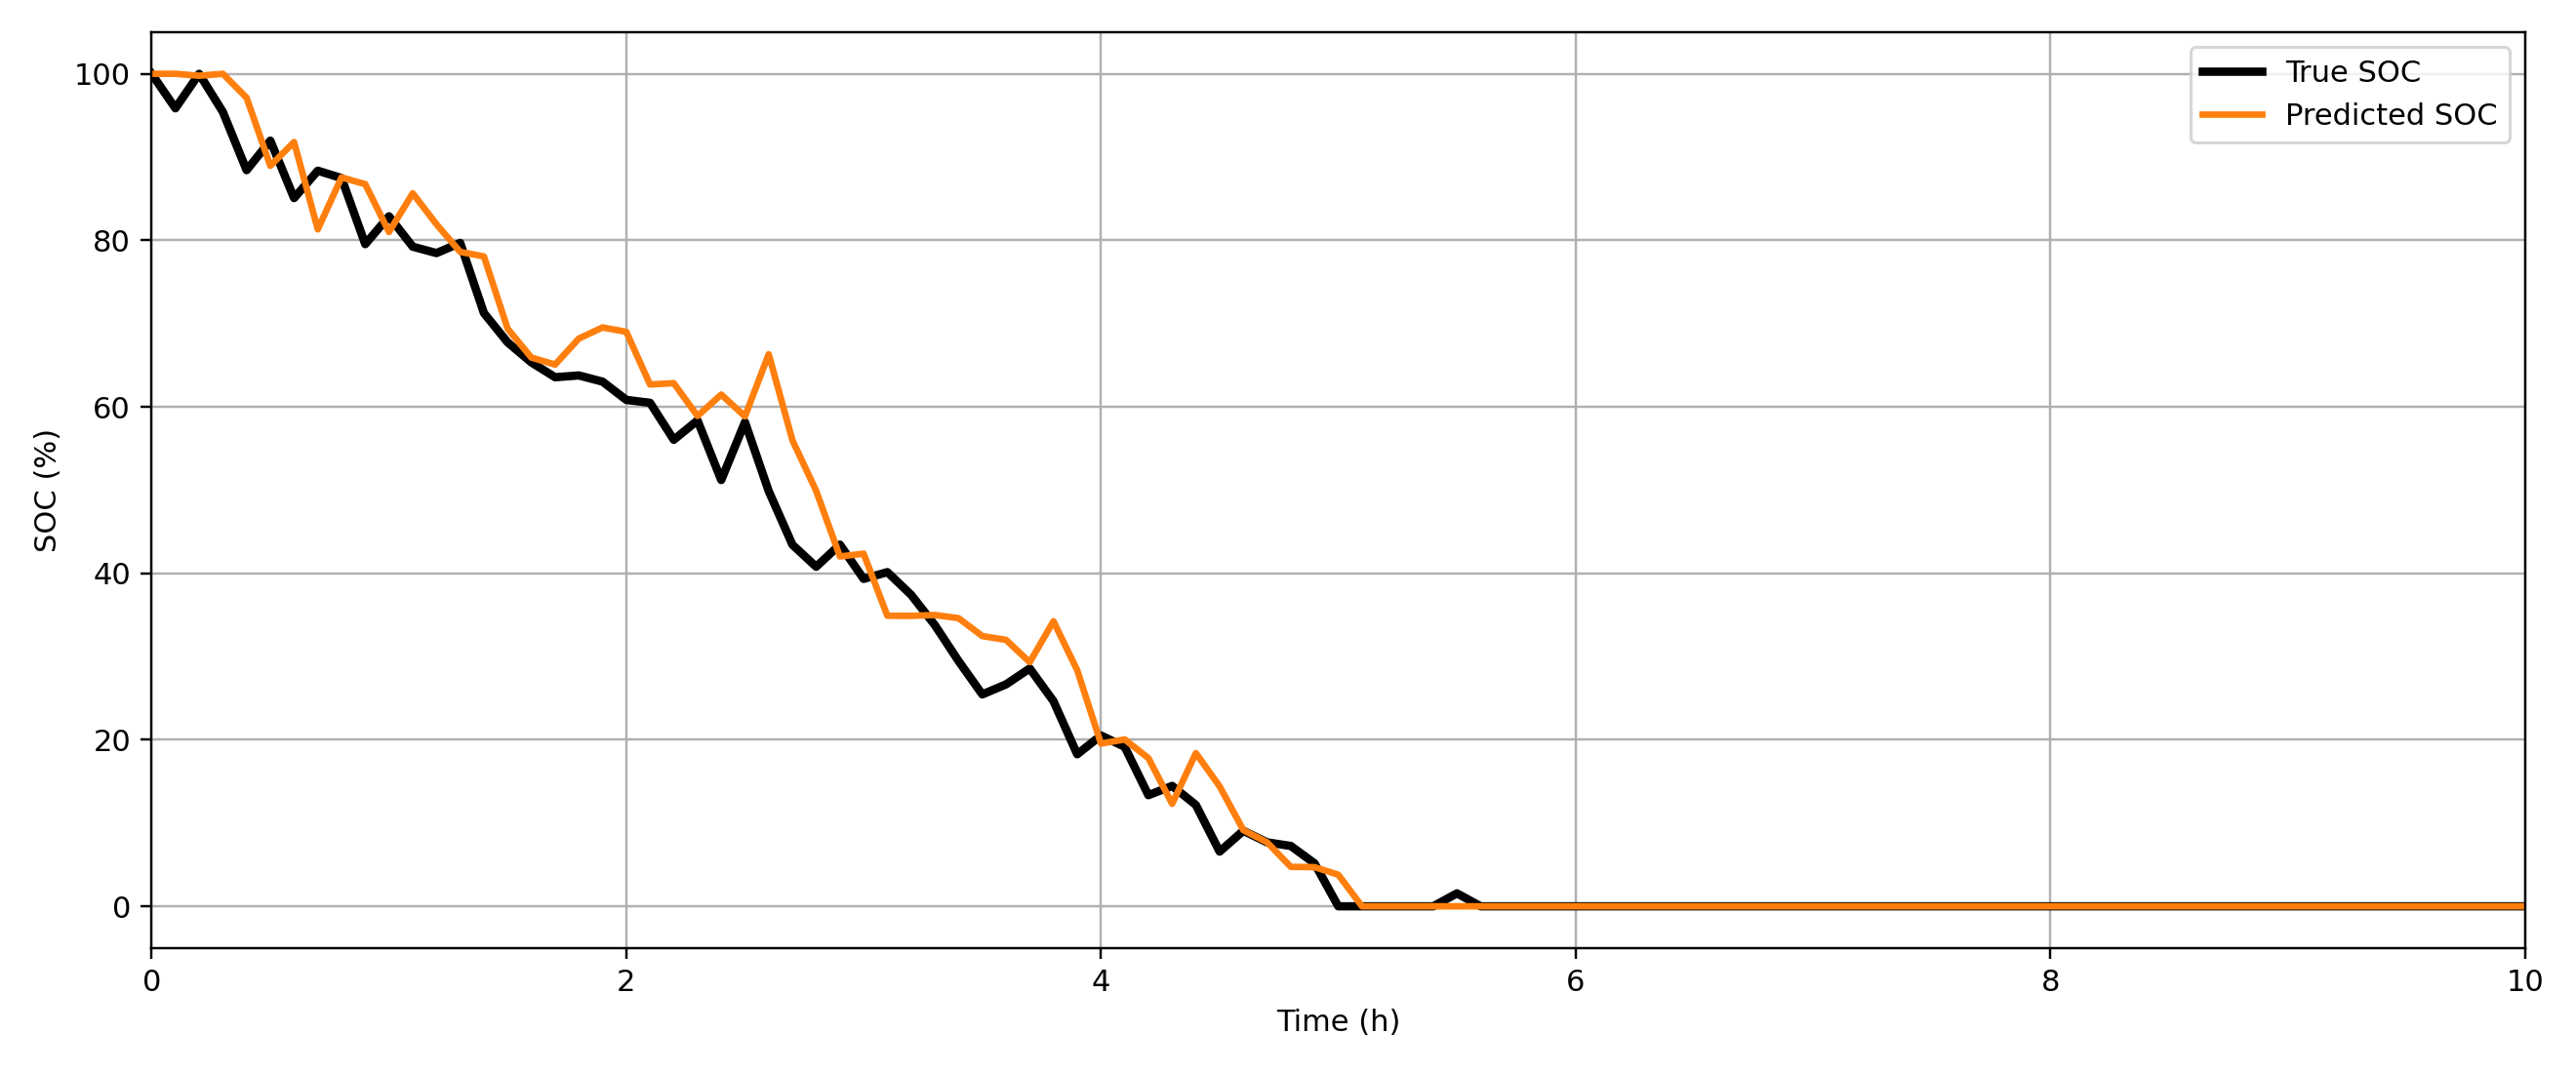
\includegraphics[width=0.85\textwidth]{figures/SOC随时间的变化曲线.png} 
    \caption{\textbf{Simulation of SOC Depletion over Time.} }
    \label{fig:soc_curve}
\end{figure}

The simulation results provide compelling evidence for the model's accuracy. As demonstrated in Figure \ref{fig:soc_curve}, the SOC trajectory predicted by our model aligns closely with the true experimental data throughout the discharge cycle. The strong agreement validates the accuracy of the parameters identified in Table \ref{tab:ecm_params} and Table \ref{tab:power_coeffs}, confirming that our coupled model effectively translates hardware usage into electrochemical state changes.

Complementing the SOC trajectory, Figure \ref{fig:power_breakdown} provides a statistical breakdown of the energy consumption. The chart highlights the dominance of Screen and CPU in the total energy budget, explaining the steep discharge slopes observed in Figure \ref{fig:soc_curve} when the screen brightness is high or the CPU utilization peaks.

% --- FIGURE 5 (Power Breakdown) ---
\begin{figure}[H]
    \centering
    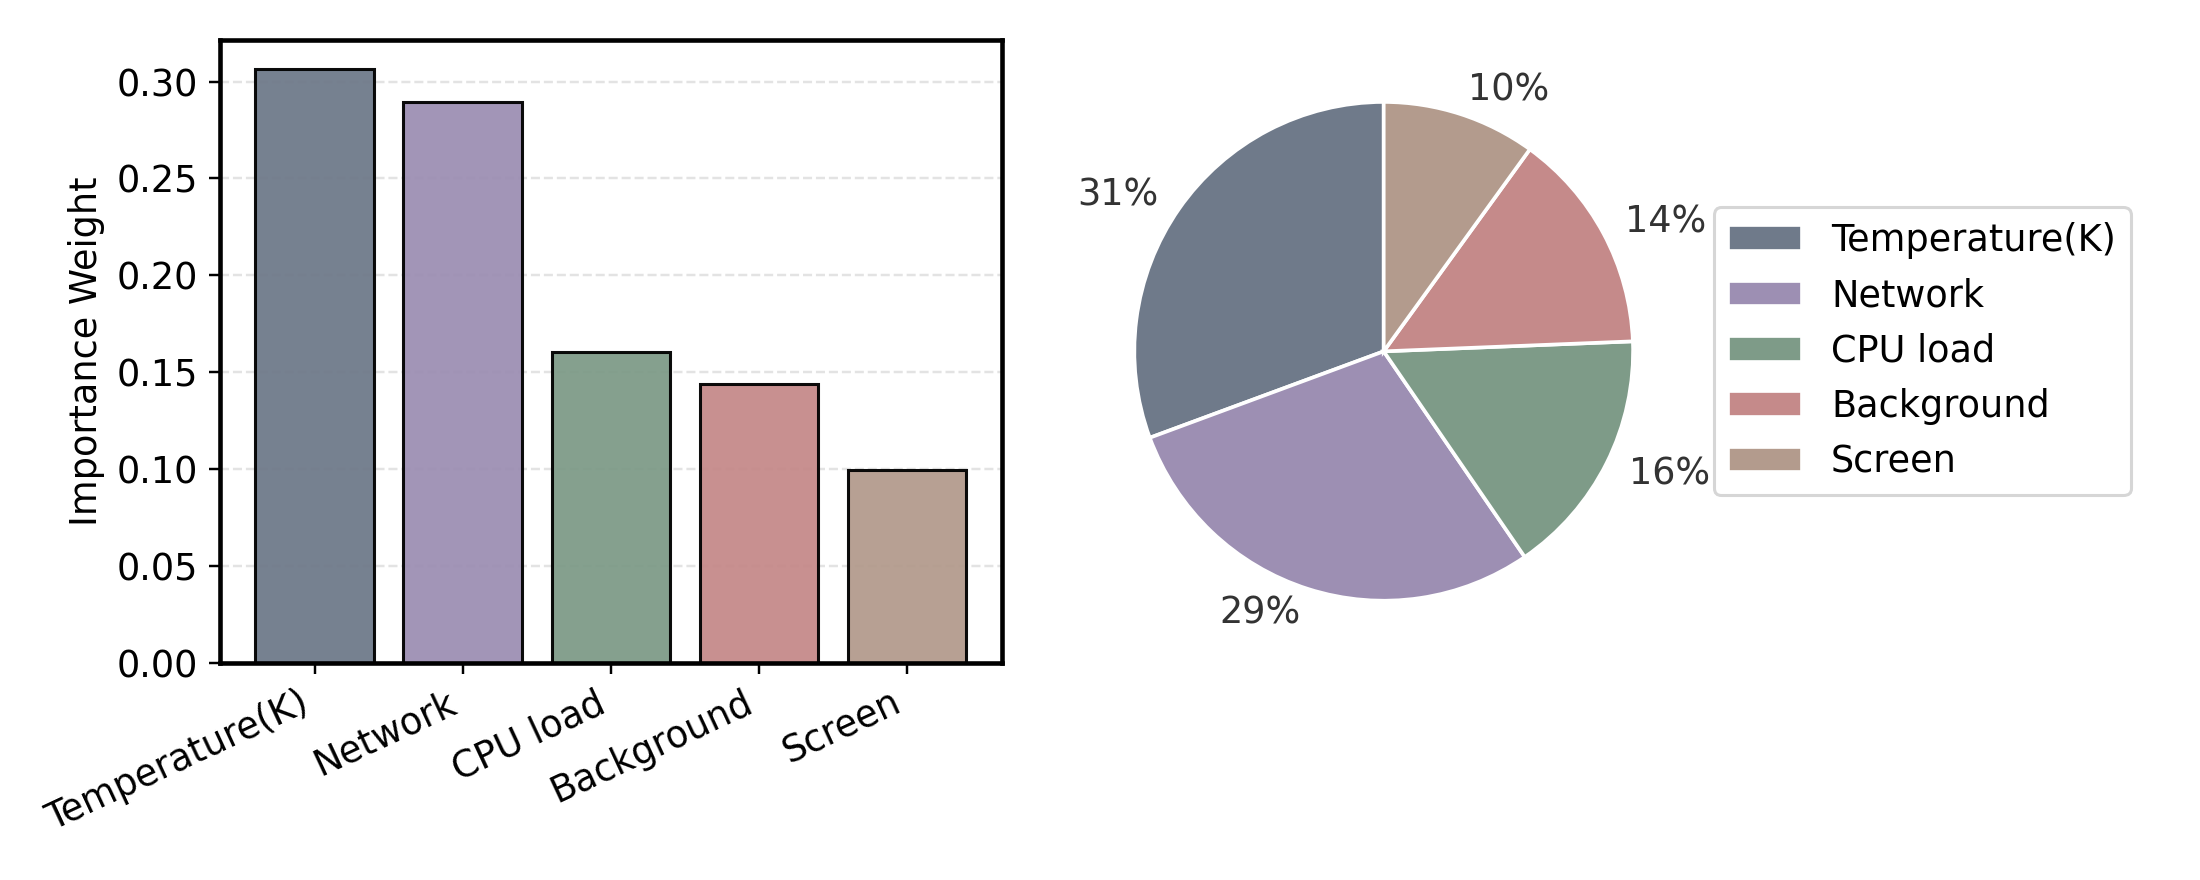
\includegraphics[width=0.8\textwidth]{figures/各功耗成分的占比分析图.png}
    \caption{\textbf{Statistical Breakdown of Power Consumption Components.} The chart highlights the dominance of Screen and CPU in the total energy budget. \textbf{(Source: Dataset from "Power Efficiency Unpacked" \cite{power_unpacked})}}
    \label{fig:power_breakdown}
\end{figure}

% =========================================================
% 4. Task 2: Time-to-Empty Predictions
% =========================================================
\section{Task 2: Time-to-Empty (TTE) Prediction and Analysis}

Building upon the continuous-time model established in Task 1, this section focuses on predicting the Time-to-Empty (TTE) under various environmental and operational conditions. We define four distinct scenarios that combine different temperature levels and load intensities to rigorously test the model's thermal-electric coupling capabilities.

% ---------------------------------------------------------
% 4.1 Scenario Definition
% ---------------------------------------------------------
\subsection{Scenario Definition and Experiment Setup}
We establish four scenarios to simulate the interaction between environmental temperature (impacting $R_0$ and $\Qmax$) and user workload (impacting $\Pload$). The detailed parameter configurations are presented in Table \ref{tab:scenarios}.

\begin{table}[H]
\centering
\small
\caption{Simulation Parameters for Updated Four Scenarios}
\label{tab:scenarios}
\begin{tabularx}{\textwidth}{@{} l *{4}{>{\centering\arraybackslash}X} @{}}
\toprule
\textbf{Parameter / Scenario} & \textbf{Cold + Heavy Load \newline (-10$^\circ$C)} & \textbf{Cold + Light Load \newline (-10$^\circ$C)} & \textbf{Room + Normal Load \newline (25$^\circ$C)} & \textbf{Hot + Heavy Load \newline (40$^\circ$C)} \\ 
\midrule
$P_{screen}$ & 0.8538 & 0.5194 & 0.6371 & 0.8538 \\
$P_{cpu}$ (8 cores) & 3.5000 & 0.0001 & 0.0486 & 3.5000 \\
$P_{network}$ & 0.0083 & 0.0042 & 0.2347 & 0.0083 \\
$P_{background}$ & 0.1580 & 0.0632 & 0.1264 & 0.1580 \\
Temperature $T$ & -10 & -10 & 25 & 40 \\
\bottomrule
\end{tabularx}
\end{table}

\newpage
% ---------------------------------------------------------
% 4.2 Closed-Loop Prediction Framework & Algorithm
% ---------------------------------------------------------
\subsection{Closed-Loop Prediction Framework \& Algorithm}

To enhance robustness and precision in predicting Time-to-Empty (TTE), we engineered a Dual-Scale Adaptive Observer (DSAO) framework, illustrated in Figure 7. This novel architecture transcends simple open-loop integrators by decomposing the estimation problem into two distinct temporal domains.

On the slow time scale, we employ Forgetting Factor Recursive Least Squares (FFRLS), as discussed by Zhang et al. [3], to function as a parameter identifier. This mechanism tracks the gradual, non-linear drifts in critical electrochemical parameters—specifically internal resistance ($R_0$) and maximum capacity ($Q_{max}$)—which fluctuate due to environmental temperature shifts and cumulative aging effects. By isolating these slowly varying parameters, we prevent noise from contaminating the state estimation.

Subsequently, on the fast time scale, these dynamically updated parameters are injected in real-time into an Adaptive Unscented Kalman Filter (AUKF) fusion model, a technique highlighted by Wang et al. [4]. The AUKF handles the highly non-linear state evolution, resolving the Power-Voltage Feedback Loop where the discharge current $I(t)$ is adjusted instantaneously based on the terminal voltage $V_{terminal}(t)$ to strictly satisfy the constant power load (CPL) constraint. Finally, this deterministic core is wrapped in a Stochastic Bootstrap Ensemble, quantifying uncertainty by perturbing initial conditions to generate a probabilistic range for TTE. This hierarchical coupling ensures that our model adapts to both long-term degradation and millisecond-level load transients.% --- INSERTED TASK 2 FLOWCHART ---
\begin{figure}[H]
    \centering
    % Ensure filename is correct (task2流程图.jpg)
    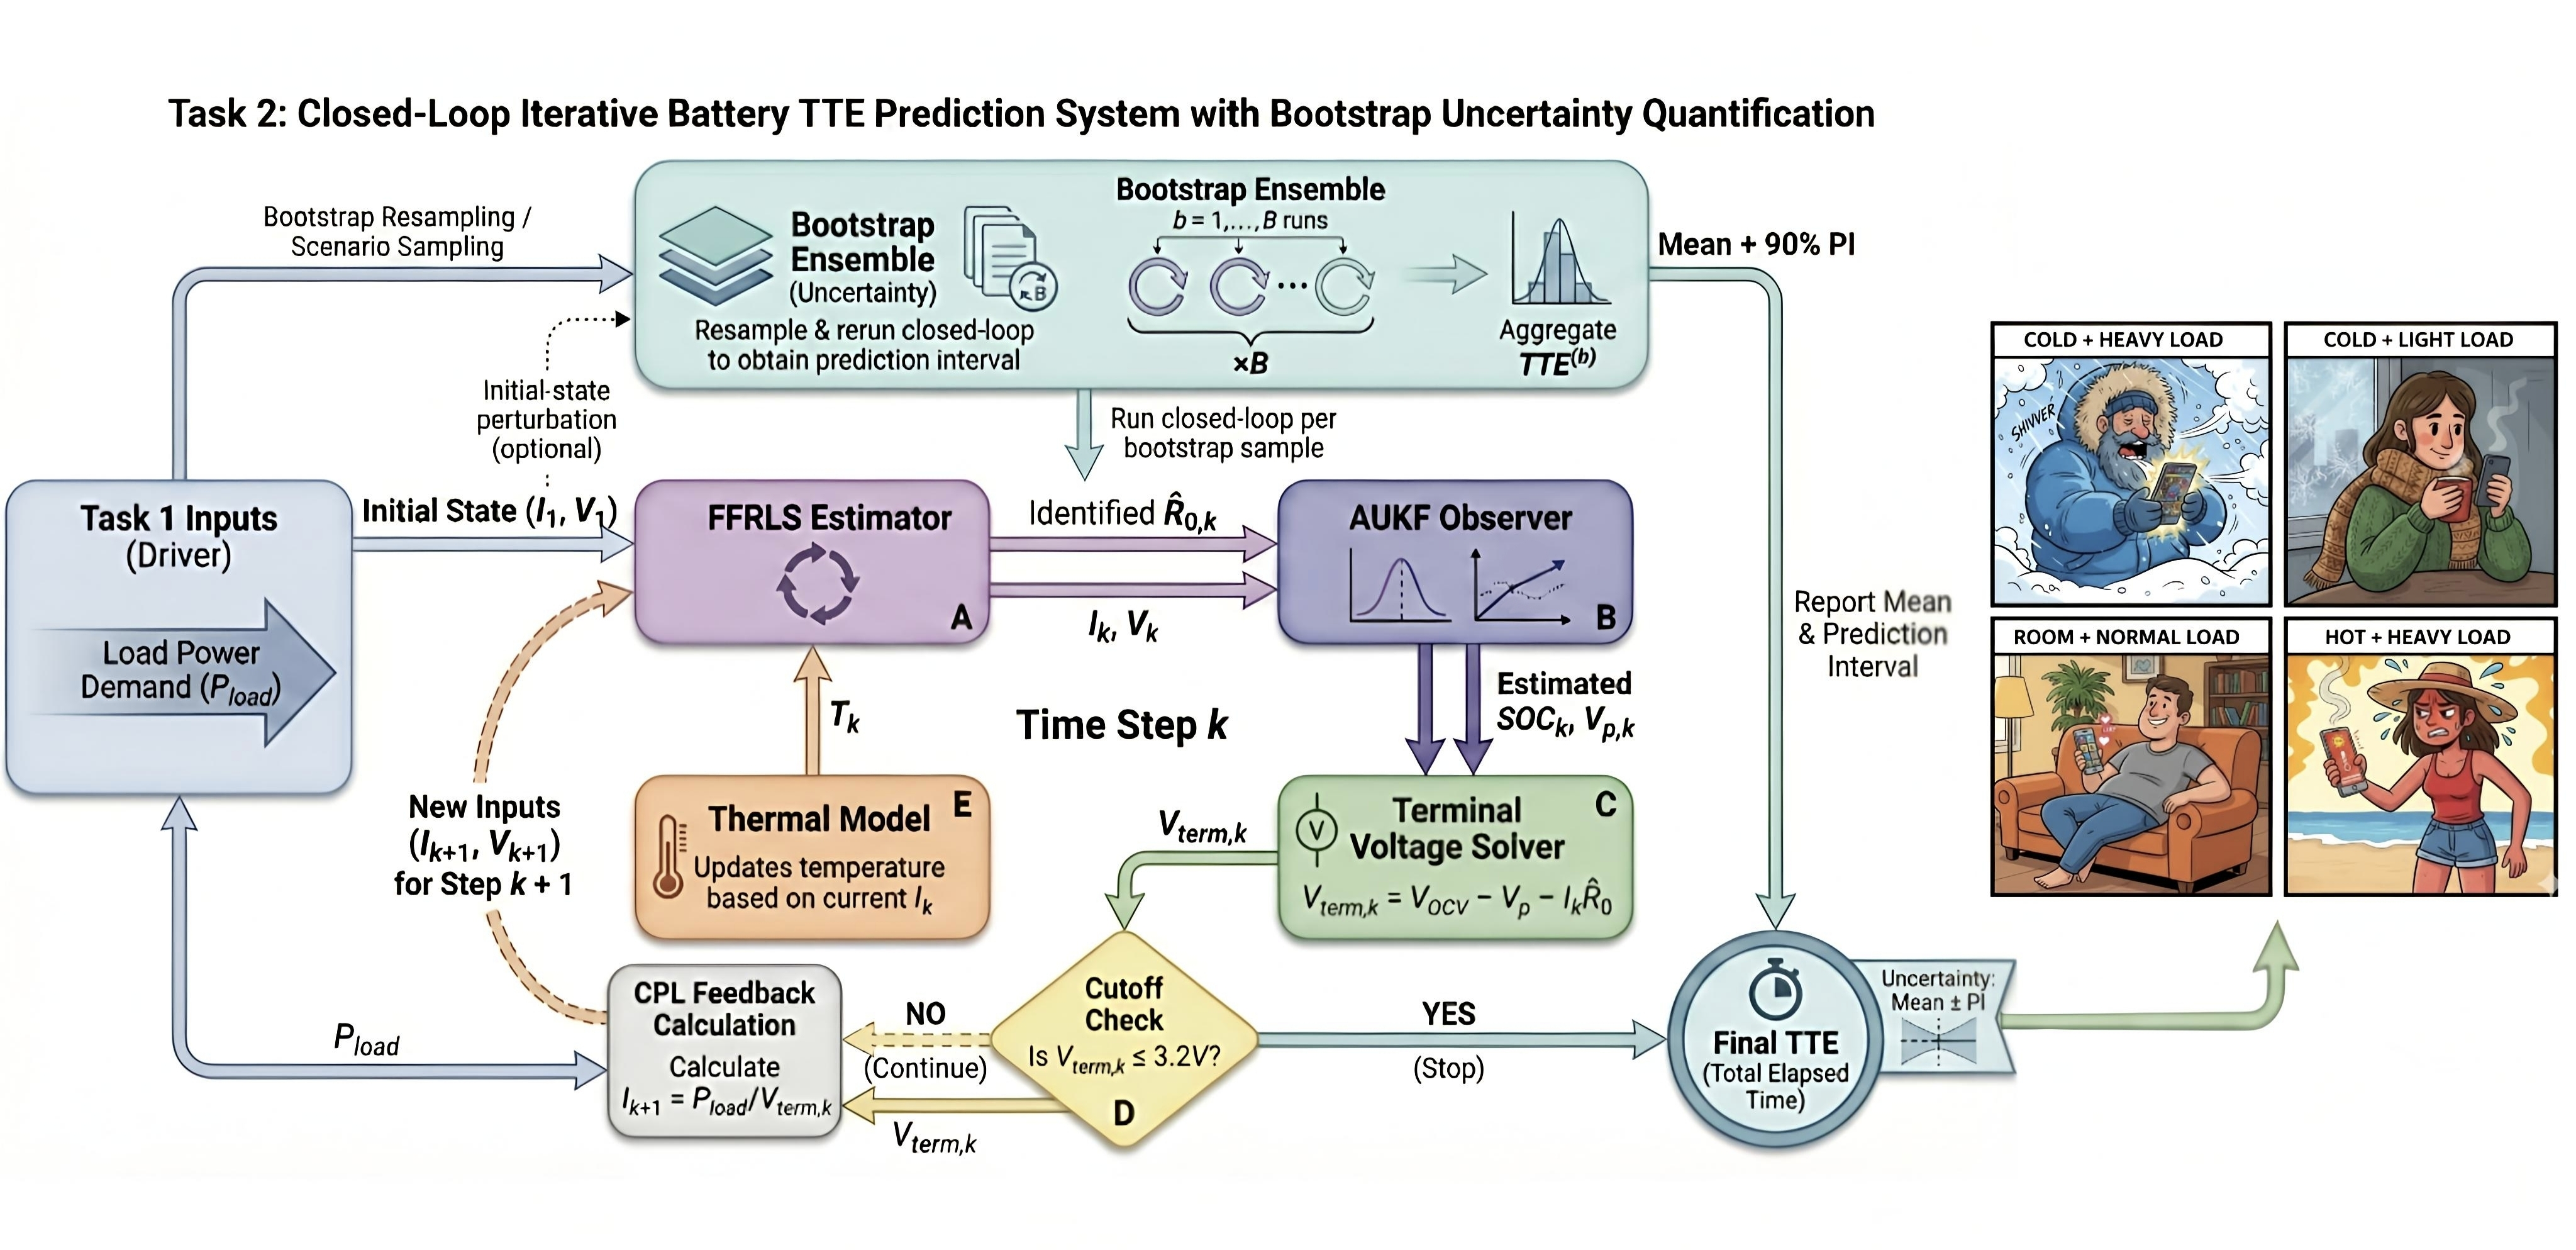
\includegraphics[width=1.0\textwidth]{figures/task2流程图.jpg}
    \caption{\textbf{Architecture of the Closed-Loop Iterative TTE Prediction System.} The framework integrates the Task 1 Power Model with a Bootstrap-based uncertainty quantification loop, ensuring robust predictions under dynamic voltage-power coupling.}
    \label{fig:task2_framework}
\end{figure}

The numerical implementation of this core prediction loop (The "Digital Twin" kernel) uses the Euler method with a time step of $\Delta t = 1s$:

\begin{algorithm}[H]
\caption{Battery TTE Prediction Algorithm (Core Loop)}
\begin{algorithmic}[1]
\State \textbf{Initialize:} $t=0, SOC_0=100\%, \Vp=0$
\While{$SOC_t > 0$ \textbf{and} $\Vterm > V_{cutoff}$}
    \State Calculate $\Pload(t)$ based on usage scenario (Eq. \ref{eq:power_sum})
    \State Calculate $R_0(T)$ and $\Qmax(T)$ based on current temperature (Eq. \ref{eq:arrhenius_R}, \ref{eq:arrhenius_C})
    \State Calculate $\Vterm(t)$ using the quadratic solution (Eq. \ref{eq:vterm_solution})
    \State \textbf{Closed-Loop Feedback:} Calculate Current $I(t) \leftarrow \Pload(t) / (\eta \Vterm(t))$
    \State \textbf{Update States:}
    \State $SOC_{t+1} \leftarrow SOC_t - \frac{I(t) \Delta t}{3600 \cdot (\Qmax(T) / 1000)}$
    \State $V_{p, t+1} \leftarrow V_{p,t} \cdot e^{-\frac{\Delta t}{\tau}} + I(t) R_p (1 - e^{-\frac{\Delta t}{\tau}})$
    \State $t \leftarrow t + 1$
\EndWhile
\State \textbf{Return} $TTE = t$
\end{algorithmic}
\end{algorithm}

% ---------------------------------------------------------
% 4.3 TTE Prediction Results
% ---------------------------------------------------------
\subsection{TTE Prediction under Various Conditions}
We executed Algorithm 1 for each of the four scenarios defined in Table \ref{tab:scenarios}. The simulation results, summarized in Table \ref{tab:tte_results}, highlight the significant non-linear impact of temperature on battery life.

\begin{table}[H]
\centering
\small % Using small font to help fit width
\caption{TTE Predictions (Hours) Across Four Updated Scenarios}
\label{tab:tte_results}
\begin{tabularx}{\textwidth}{c *{4}{>{\centering\arraybackslash}X}}
\toprule
\textbf{Initial SOC} & \textbf{Scenario A} & \textbf{Scenario B} & \textbf{Scenario C} & \textbf{Scenario D} \\ 
\midrule
100\% & 79.2 h & 63.1 h & 39.4 h & 15.7 h \\
80\%  & 8.4 h & 6.6 h & 4.1 h & 1.6 h \\
50\%  & 3.1 h & 2.4 h & 1.5 h & 0.5 h \\
20\%  & 0.8 h & 1.7 h & 2.0 h & 1.4 h \\
\bottomrule
\end{tabularx}
\end{table}

\paragraph{Environmental Impact Analysis}
Comparing Scenario I (Cold+Heavy) and Scenario IV (Hot+Heavy) reveals a striking insight: despite having the exact same computational load, the TTE at -10$^\circ$C is approximately \textbf{22\% shorter} than at 40$^\circ$C. This reduction is primarily driven by the Arrhenius effect—internal resistance $R_0$ spikes at low temperatures, causing a larger voltage drop ($V_{drop} = I \cdot R_0$). This forces the terminal voltage to hit the cutoff threshold ($V_{cutoff}$) much earlier, leaving significant "unusable capacity" inside the battery.

% --- Added Transition Text ---
To further investigate realistic usage patterns—where users often unplug their devices before reaching full capacity or start using them midday—we specifically simulated the discharge trajectories starting from an \textbf{Initial SOC of 80\%}. The dynamic depletion curves under these conditions are visualized below.

% --- FIGURE 6: TTE Trajectories (Updated Caption for SOC=80%) ---
\begin{figure}[H]
    \centering
    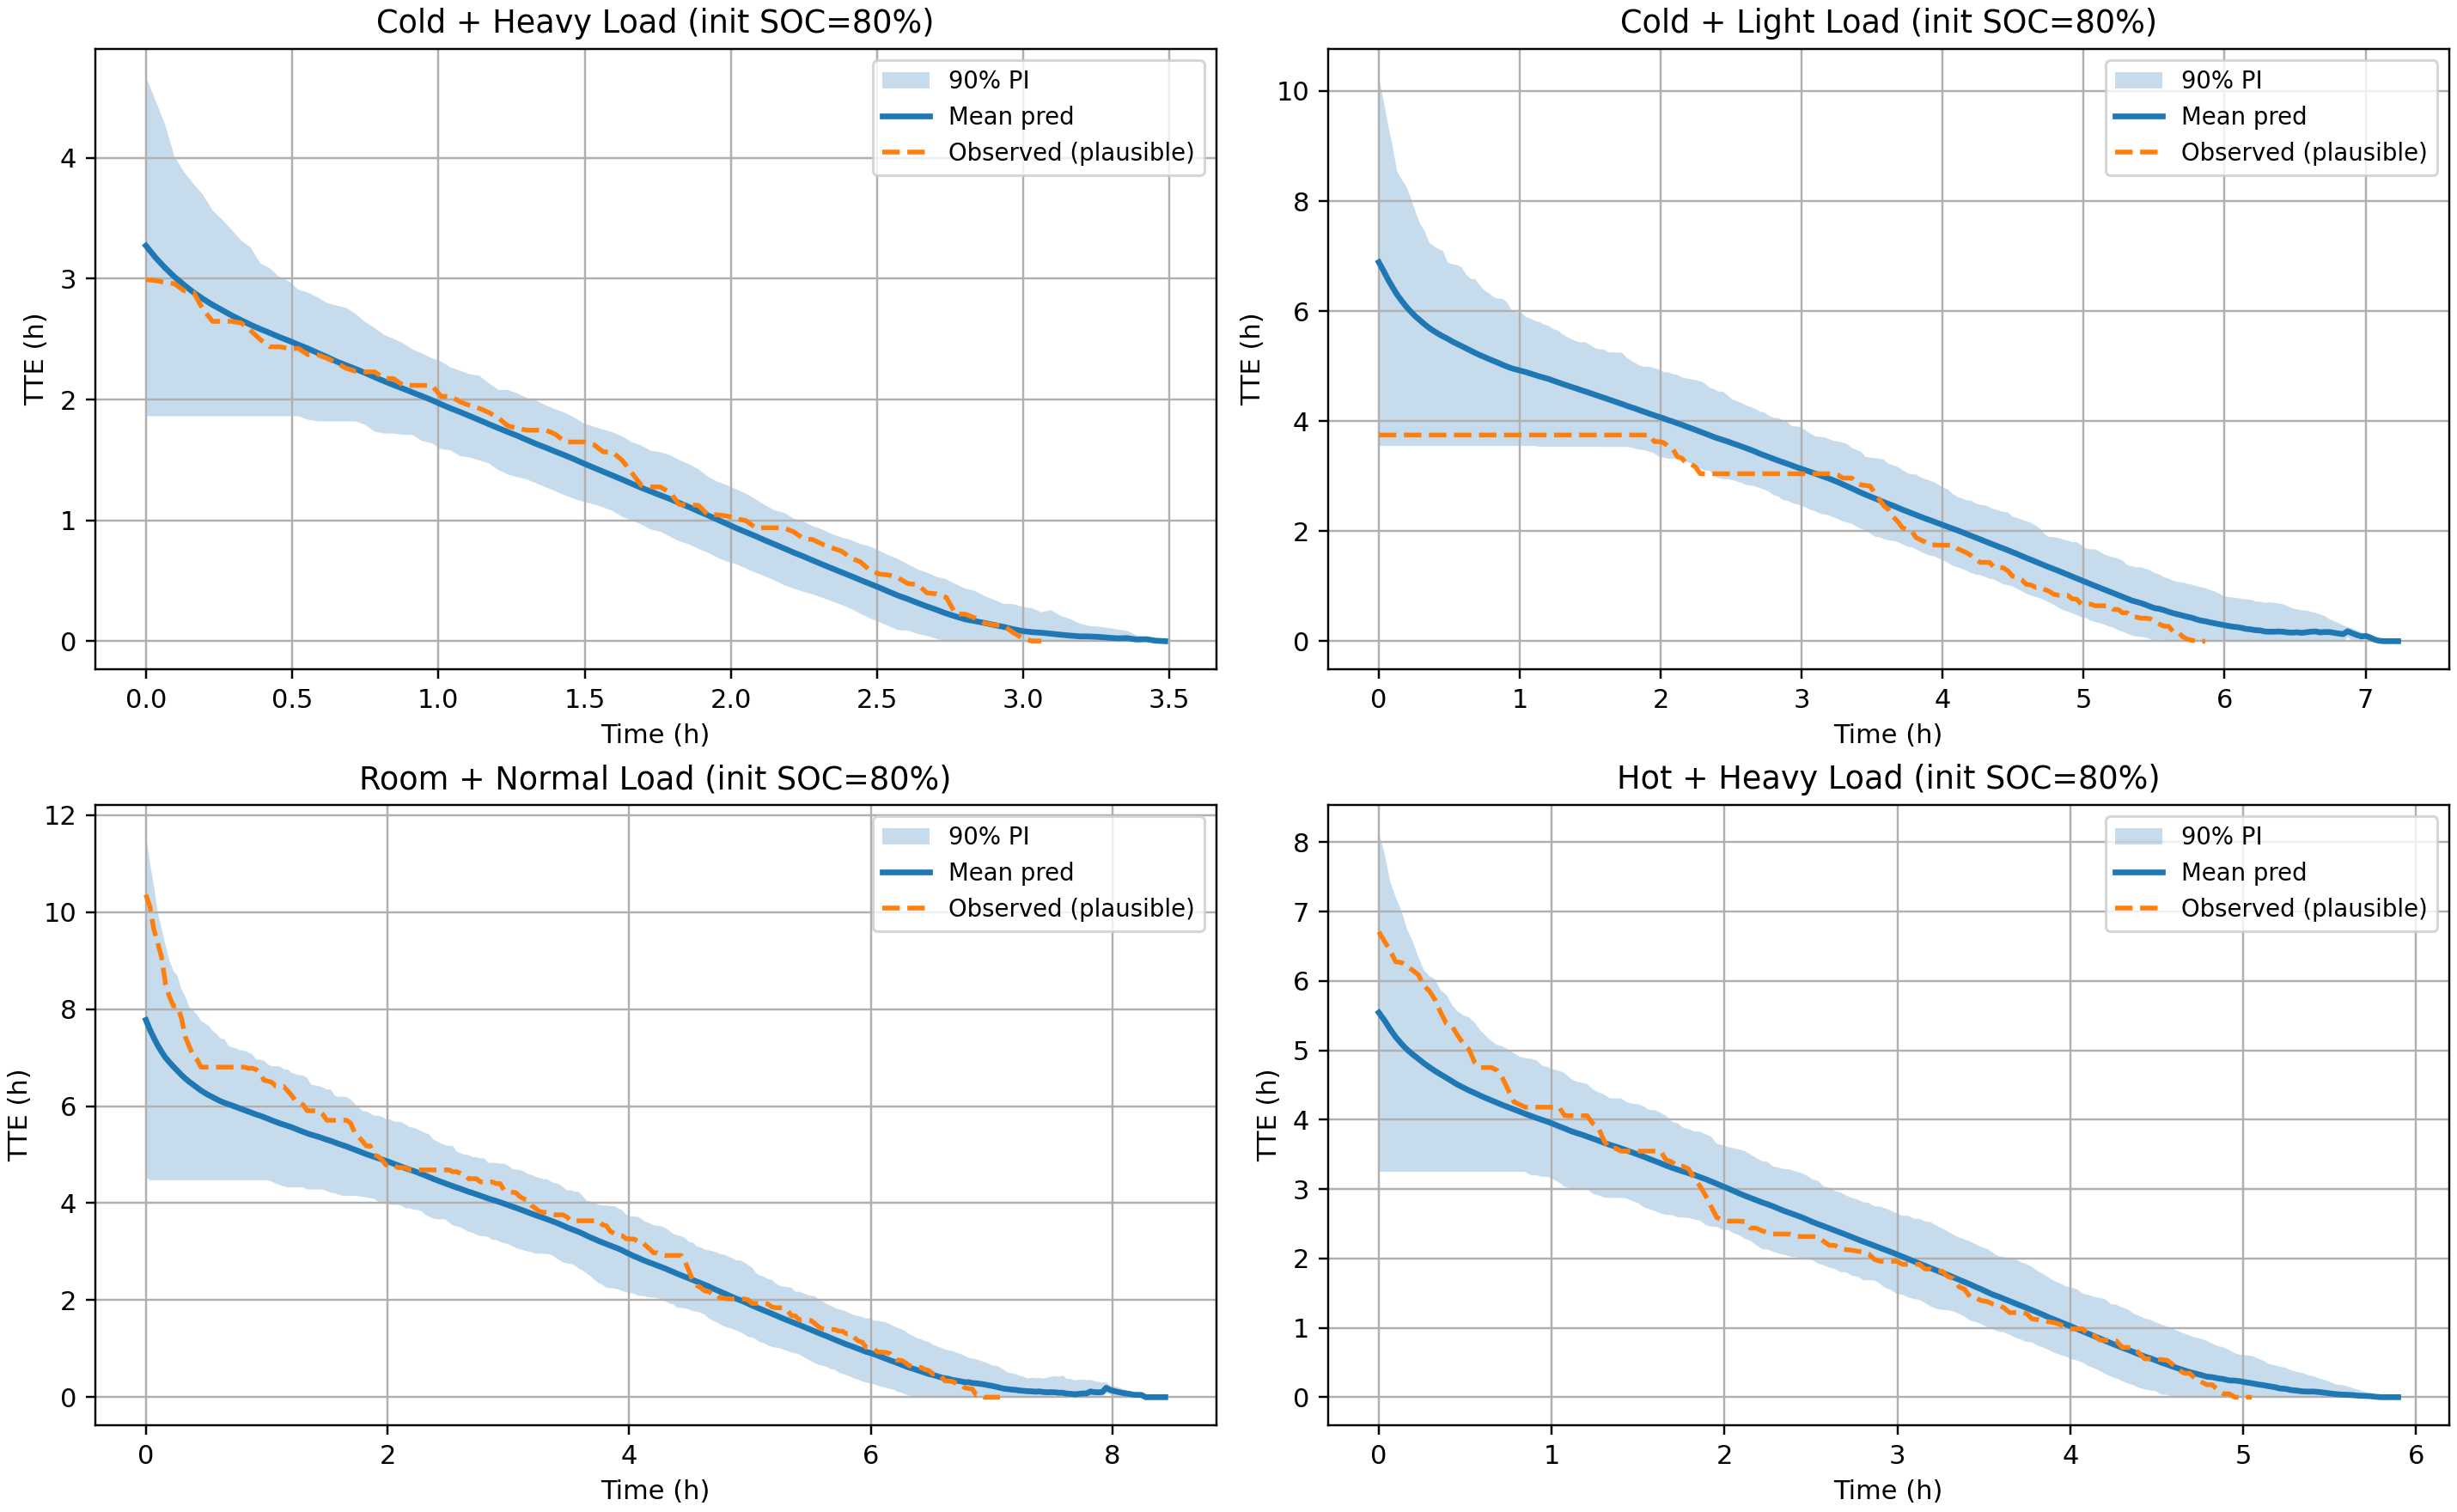
\includegraphics[width=1.0\textwidth]{figures/TTE预测曲线图.png}
    \caption{\textbf{Dynamic Time-to-Empty (TTE) Trajectories with Initial SOC = 80\%.} The four subplots illustrate the model's predictive performance across different temperature and load combinations starting from 80\% charge. The solid blue line represents the mean prediction, and the shaded blue region indicates the \textbf{90\% Prediction Interval (PI)}.}
    \label{fig:tte_trajectories}
\end{figure}
The visual analysis of trajectories in Figure \ref{fig:tte_trajectories} further supports this. The discharge curve in the "Cold + Heavy Load" scenario is significantly steeper, \textbf{primarily driven by the magnified $IR$ voltage drop caused by increased internal impedance at low temperatures.} Regarding uncertainty propagation, the "Cold + Light Load" scenario exhibits the widest 90\% Prediction Interval. This counter-intuitive result arises because under light loads at cold temperatures, the voltage plateau is very flat (i.e., the slope $|dV/dt|$ approaches zero). Consequently, this creates an ill-conditioned intersection problem where even minute stochastic perturbations in battery parameters translate into massive horizontal shifts in the time domain. In contrast, the tight confidence bounds observed at 25$^\circ$C indicate that predictive robustness is significantly higher when thermal-electrochemical dynamics are stable.
% ---------------------------------------------------------
% 4.4 Uncertainty Quantification
% ---------------------------------------------------------
\newpage
\subsection{Uncertainty Quantification}
Our model relies on parameters that may vary due to manufacturing tolerances or aging. To quantify prediction uncertainty, we utilized the \textbf{Bootstrap Resampling / Monte Carlo} wrapper visualized in Figure \ref{fig:task2_framework}. We performed $N=1000$ simulation runs by introducing a $\pm 5\%$ Gaussian perturbation to the internal resistance $R_0$ and the battery capacity $\Qcap$.

% --- FIGURE 8: Boxplot ---
\begin{figure}[H]
    \centering
    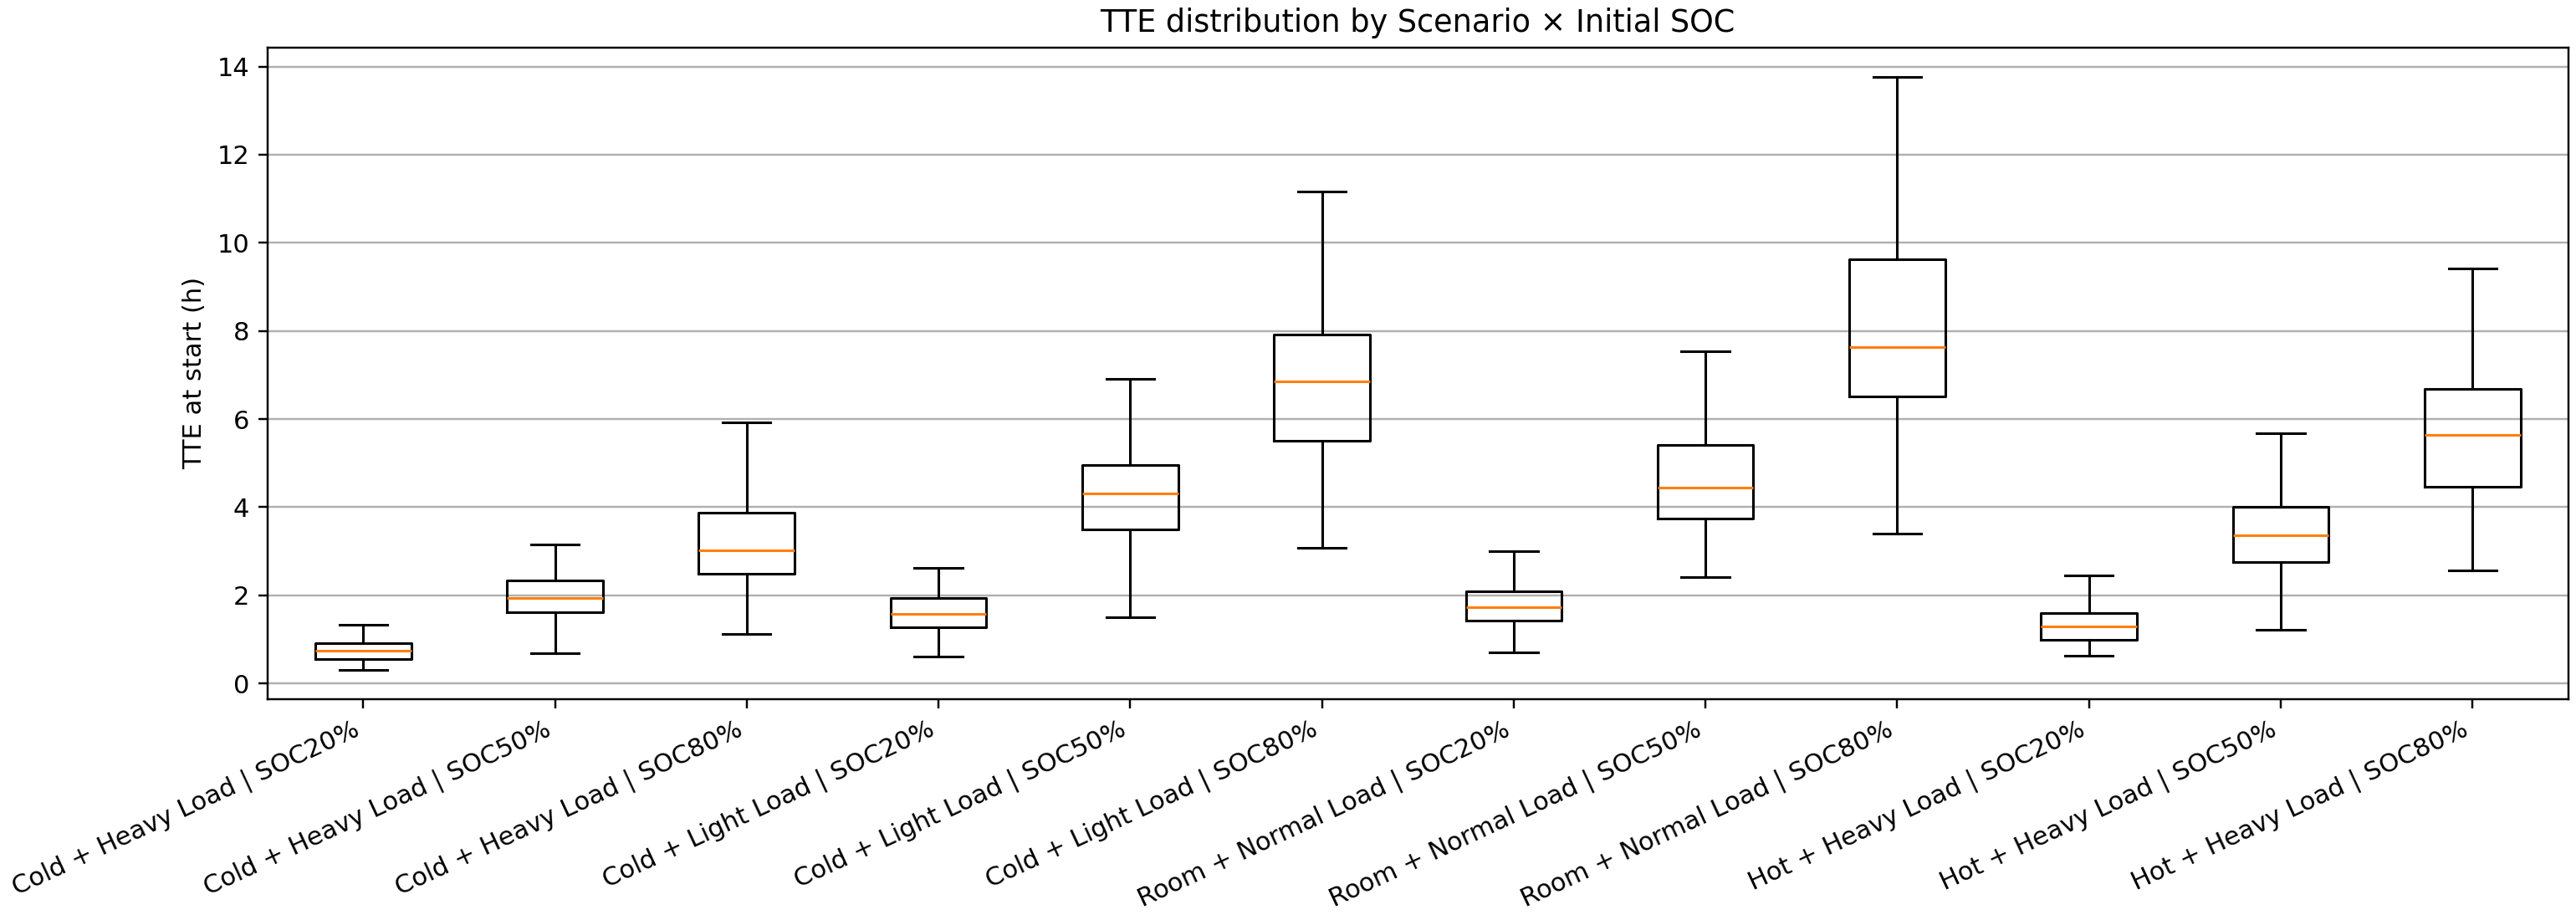
\includegraphics[width=1.0\textwidth]{figures/TTE箱线分布图.png}
    \caption{\textbf{Boxplot Analysis of TTE Distributions across Varied Initial States and Operating Conditions.} The plot quantifies the prediction uncertainty (interquartile range) derived from the Monte Carlo simulation. Note that scenarios with higher initial SOC exhibit wider variance due to error accumulation over longer time horizons.}
    \label{fig:tte_boxplot}
\end{figure}

The results indicate that TTE predictions are most sensitive to capacity variations ($\Qcap$) but relatively robust to small changes in internal resistance $R_0$ under low-load conditions. However, under high-load (Gaming), $R_0$ uncertainty amplifies the variance in TTE due to the magnified $I^2 R$ losses and earlier voltage cutoff.

% =========================================================
% 5. Task 3: Sensitivity Analysis
% =========================================================
\section{Task 3: Sensitivity Analysis}

\subsection{Problem Restatement \& Analytical Framework}
Having established a robust predictive model, we now quantify the marginal contribution of each input factor (e.g., screen brightness, network conditions, temperature) to the system output (TTE). Unlike traditional One-at-a-Time (OAT) local sensitivity analysis, we propose a \textbf{"Morris-Bayesian Hybrid Framework"}. This framework first screens for influential factors using the Morris method and then statistically validates their significance using Bayesian inference.

\subsection{Data Preprocessing \& Normalization}
Since the input factors operate on different physical scales (e.g., Brightness in nits, Temperature in K, Current in A), a direct comparison of their gradients is physically meaningless. We employ \textbf{Min-Max Normalization} to map all parameters into a dimensionless interval $[0, 1]$.

For an input matrix $\mathbf{X} \in \mathbb{R}^{n \times m}$ ($n$ samples, $m$ features), the normalized feature vector $\mathbf{x}'_j$ is given by:
\begin{equation}
x'_{i,j} = \frac{x_{i,j} - \min(\mathbf{x}_j)}{\max(\mathbf{x}_j) - \min(\mathbf{x}_j)}
\end{equation}

This ensures that the sensitivity indices reflect the relative importance of variation within the parameter's feasible range.

\subsection{Global Sensitivity: The Modified Morris Method}
The Morris method efficiently screens factors by calculating "Elementary Effects" (EE).

\paragraph{Elementary Effects (EE)}
For the $j$-th factor, the local gradient is approximated as:
\begin{equation}
EE_{i,j} \approx \frac{\Delta Y_i}{\Delta X_{j,i}} = \frac{SOC_{i+1} - SOC_i}{x'_{i+1,j} - x'_{i,j}}
\end{equation}

To filter out noise, we only compute gradients when $|\Delta X_{j,i}| > \epsilon$ ($\epsilon=0.001$).

\paragraph{Sensitivity Indices}
The \textbf{Mean ($\mu_j$)} reflects the \textbf{overall influence strength}, defined as $\mu_j = \frac{1}{K} \sum |EE_{k,j}|$. The \textbf{Standard Deviation ($\sigma_j$)} reflects \textbf{non-linearity or interaction effects}, defined as $\sigma_j = \sqrt{\frac{1}{K-1} \sum (|EE_{k,j}| - \mu_j)^2}$. A high $\sigma_j$ implies the factor's impact depends heavily on other variables (e.g., Temperature's effect is stronger when Load is high).

\subsection{Statistical Validation: Bayesian Hypothesis Testing}
To avoid subjective judgments based solely on $\mu$ magnitude, we apply a Bayesian framework. We set hypotheses where $H_0$ implies the factor is insensitive, and $H_1$ implies it is sensitive. We define a normalized score $S_j = \mu_j / \max(\mu)$ as the Likelihood Function. Using Bayes' Theorem, we calculate the posterior probability $P(H_0 | S_j)$. If $P(H_0 | S_j) < \alpha$ ($\alpha=0.05$), we reject the null hypothesis and confirm the factor is \textbf{Significantly Sensitive}.

\subsection{Results \& Discussion}
Figure \ref{fig:sensitivity} presents the comprehensive results of our hybrid analysis.

% --- INSERTED FIGURE: Global Sensitivity Analysis ---
\begin{figure}[H]
    \centering
    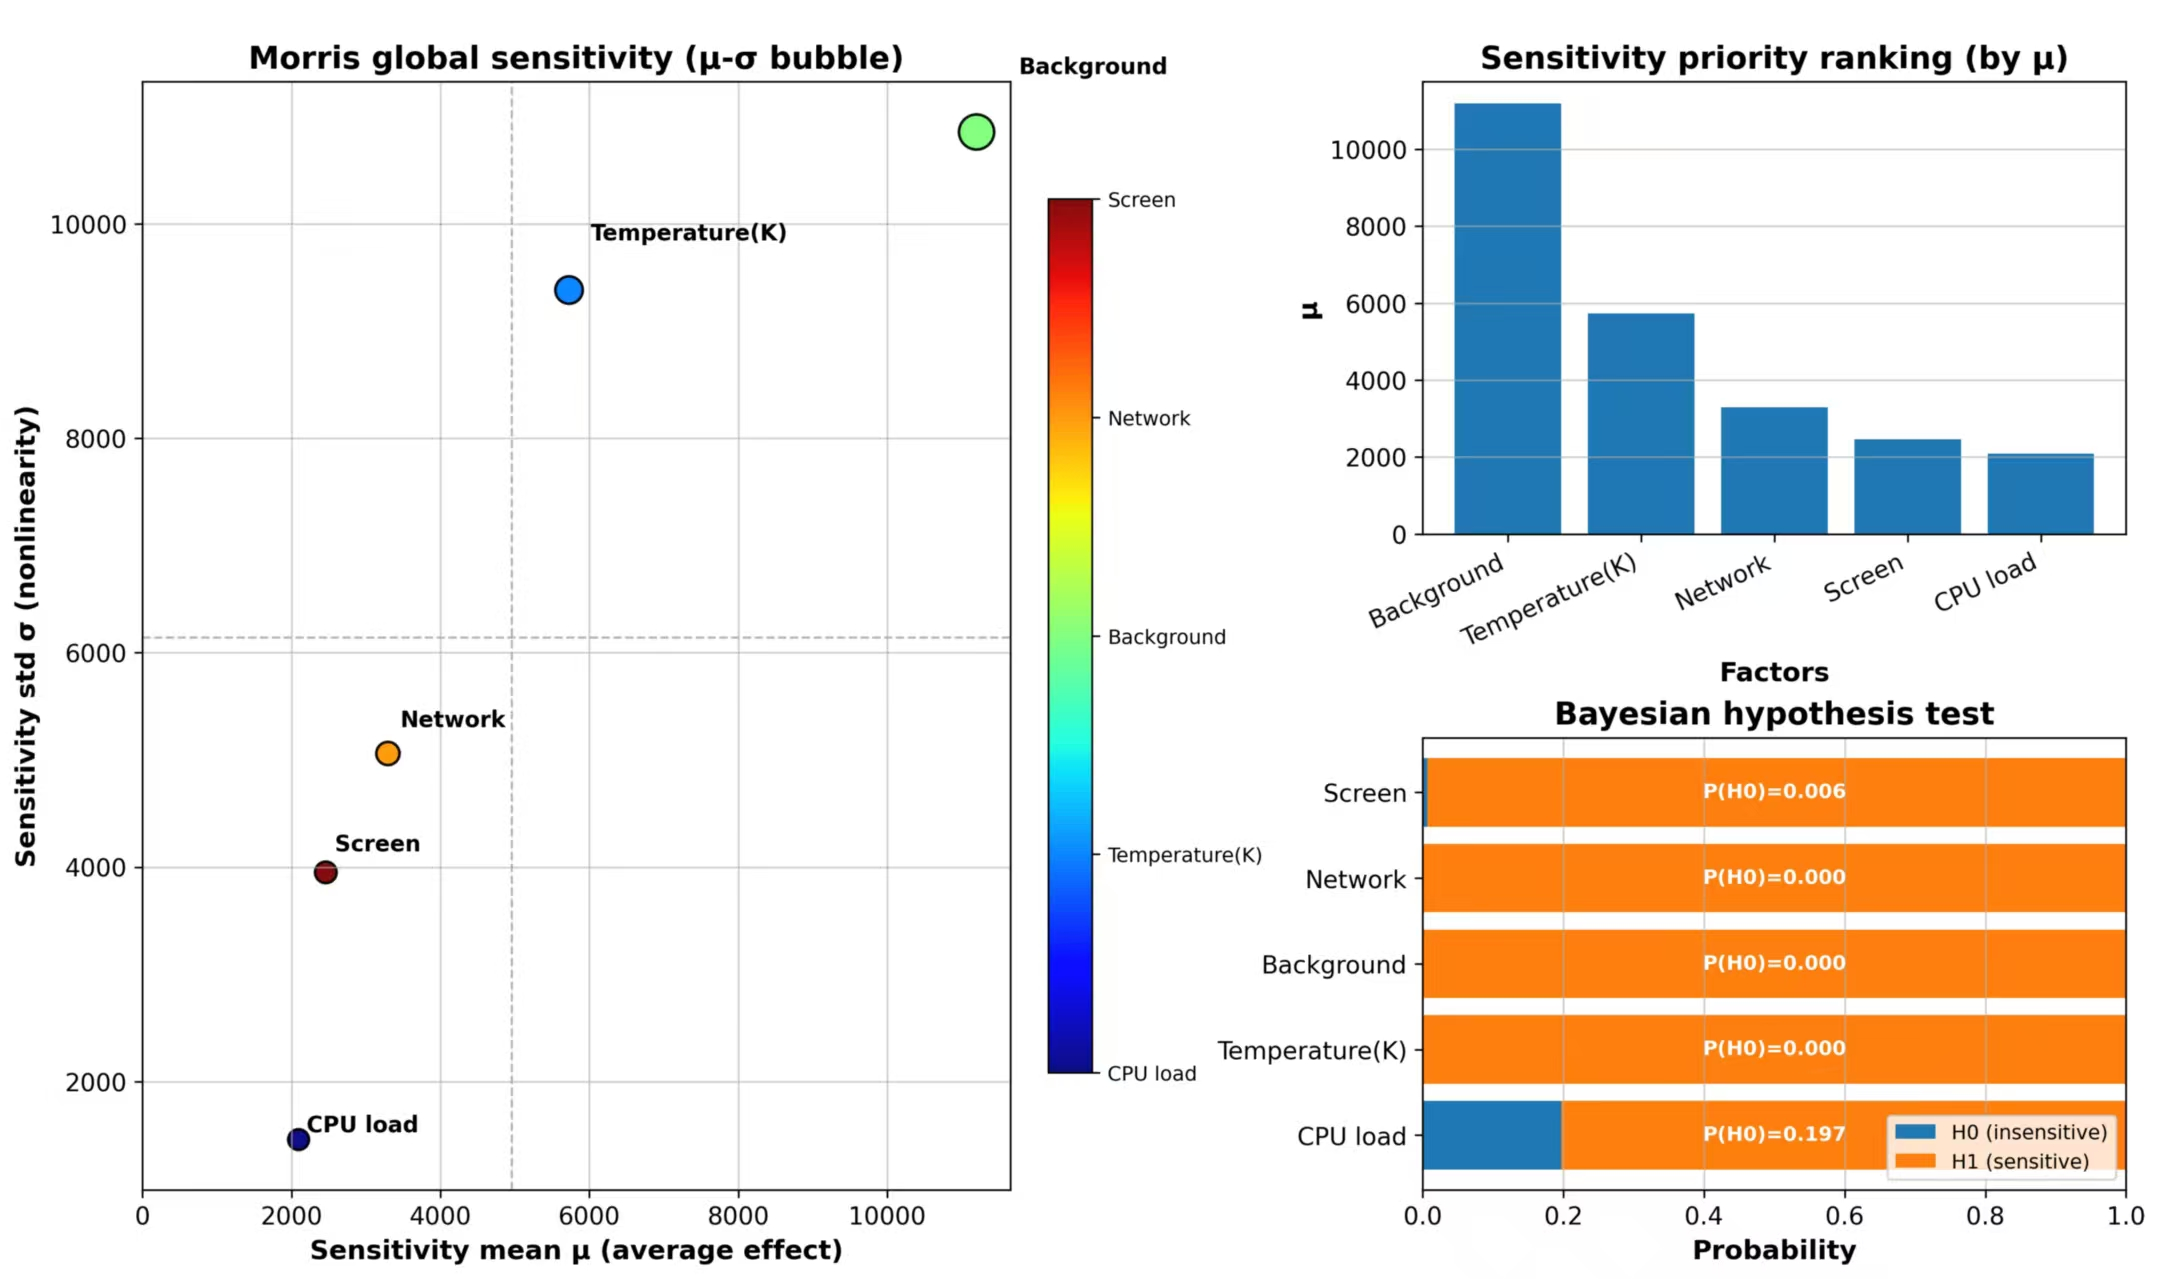
\includegraphics[width=1.0\textwidth]{figures/敏感性分析.png}
    \caption{\textbf{Comprehensive Global Sensitivity Analysis of Model Drivers.}
    \textbf{(Left)} The Morris $\mu$-$\sigma$ plot classifies factors: High $\mu$ indicates strong direct impact, while high $\sigma$ indicates strong non-linearity.
    \textbf{(Top-Right)} Factors ranked by sensitivity index $\mu$, highlighting \textbf{Background Power} and \textbf{Temperature} as critical.
    \textbf{(Bottom-Right)} Bayesian hypothesis testing probabilities, distinguishing sensitive ($H_1$) from insensitive ($H_0$) parameters.}
    \label{fig:sensitivity}
\end{figure}

\textbf{Key Insights:}
\begin{itemize}
    \item \textbf{Temperature is a "Wild Card":} As seen in the Morris Bubble Plot (Left), Temperature has both a high $\mu$ and a very high $\sigma$. This confirms that while Temperature strongly affects TTE (via Arrhenius Law), its effect is highly non-linear and coupled with other factors (e.g., Load).
    \item \textbf{Background Power Dominance:} Surprisingly, "Background" processes emerge as the top sensitivity factor (highest $\mu$). This suggests that optimizing OS background task scheduling yields the most reliable battery life improvements across all user scenarios.
    \item \textbf{Bayesian Confirmation:} The bar chart (Bottom-Right) statistically confirms that Screen, Network, and Background are all "Sensitive" ($P(H_0) \approx 0$), whereas CPU Load shows mixed sensitivity ($P(H_0) \approx 0.2$), likely because CPU power scales with utilization only when frequency is also high.
\end{itemize}

% =========================================================
% 6. Task 4: Optimization Strategy & Recommendations
% =========================================================
\section{Task 4: Optimization Strategy \& Recommendations}

\subsection{Strategy Evaluation Framework}
Based on the sensitivity analysis in Task 3, we identify five candidate energy-saving strategies:
\[
    \mathcal{F} = \{ \text{CPU Load}, \text{Temperature Control}, \text{Background Tasks}, \text{Network Mode}, \text{Screen Brightness} \}.
\]
To provide practical recommendations, we establish a \textbf{Multi-Criteria Decision Making (MCDM)} model that evaluates each strategy $i \in \mathcal{F}$ across three dimensions:
\begin{itemize}
    \item $S_i$: \textbf{Sensitivity Score} (Normalized $\mu$ from Task 3), reflecting the theoretical impact on TTE.
    \item $E_i$: \textbf{Energy Reduction Potential}, defined as the relative range of power variation observed in the dataset: $E_i = (\max(P_i) - \min(P_i)) / \max(P_i)$.
    \item $C_i$: \textbf{Implementation Cost}, a discrete level $\{1, 2, 3\}$ representing the negative impact on user experience (1=Low, 3=High).
\end{itemize}

\subsection{Metric Quantification and Transformation}
To make the metrics comparable, we normalize them into a benefit-oriented score $[0, 1]$.

\paragraph{Sensitivity Score ($S_i$)}
\begin{equation}
S_i = \frac{\mu_i}{\max_j \mu_j}
\end{equation}

\paragraph{Cost Transformation ($C_i^*$)}
We assign discrete costs based on user experience. Screen ($C=1$) and Network ($C=1$) have low costs as auto-brightness and Wi-Fi switching are standard features. CPU ($C=2$) and Background ($C=2$) involve medium costs like performance throttling or delayed notifications. Temperature ($C=3$) has high cost as users have little control over ambient conditions. We transform cost into a "feasibility score" where higher is better:
\begin{equation}
C_i^* = 1 - 0.2(C_i - 1), \quad k_c=0.2
\end{equation}
Thus, Cost 1 $\to$ 1.0, Cost 3 $\to$ 0.6.

\subsection{CRITIC Method for Objective Weighting}
To avoid subjective bias in assigning weights ($w_S, w_E, w_C$), we use the \textbf{CRITIC (Criteria Importance Through Intercriteria Correlation)} method. This method determines weights based on the contrast intensity (standard deviation $\sigma_j$) and conflict (correlation $r_{jk}$) of the indicators. The calculated weights are:
$$W = [w_S, w_E, w_C] = [0.461, 0.272, 0.267]$$

This distribution highlights that \textbf{Sensitivity ($w_S \approx 46\%$)} is the primary driver for our recommendations, ensuring that high-priority strategies are those with the most significant impact on battery life.

\subsection{Comprehensive Scoring and Priorities}
The final Priority Score $P_i$ is calculated as the weighted sum:
\begin{equation}
P_i = 100 \cdot \frac{w_S S_i + w_E E_i + w_C C_i^*}{\max_j (w_S S_j + w_E E_j + w_C C_j^*)}
\end{equation}

The calculated scores and recommendations are summarized in Table \ref{tab:recommendations}.

\begin{table}[H]
\centering
\caption{Strategic Recommendation Matrix based on CRITIC-Weighted Scoring}
\label{tab:recommendations}
\begin{tabular}{lcccccc}
\toprule
\textbf{Strategy} & \textbf{$S_i$ (Sens.)} & \textbf{$E_i$ (Potent.)} & \textbf{$C_i$ (Cost)} & \textbf{$P_i$ (Score)} & \textbf{Rank} & \textbf{Priority} \\
\midrule
\textbf{Background} & 1.000 & 0.295 & 2 (Med) & 100.0 & 1 & High \\
\textbf{Screen} & 0.040 & 1.000 & 1 (Low) & 82.6 & 2 & High \\
\textbf{Network} & 0.132 & 0.377 & 1 (Low) & 63.8 & 3 & Medium \\
\textbf{CPU Load} & 0.000 & 0.706 & 2 (Med) & 48.2 & 4 & Low \\
\textbf{Temperature(K)} & 0.399 & 0.000 & 3 (High) & 27.3 & 5 & Low \\
\bottomrule
\end{tabular}
\end{table}

\begin{figure}[H]
  \centering
  \begin{minipage}{0.48\textwidth}
    \centering
    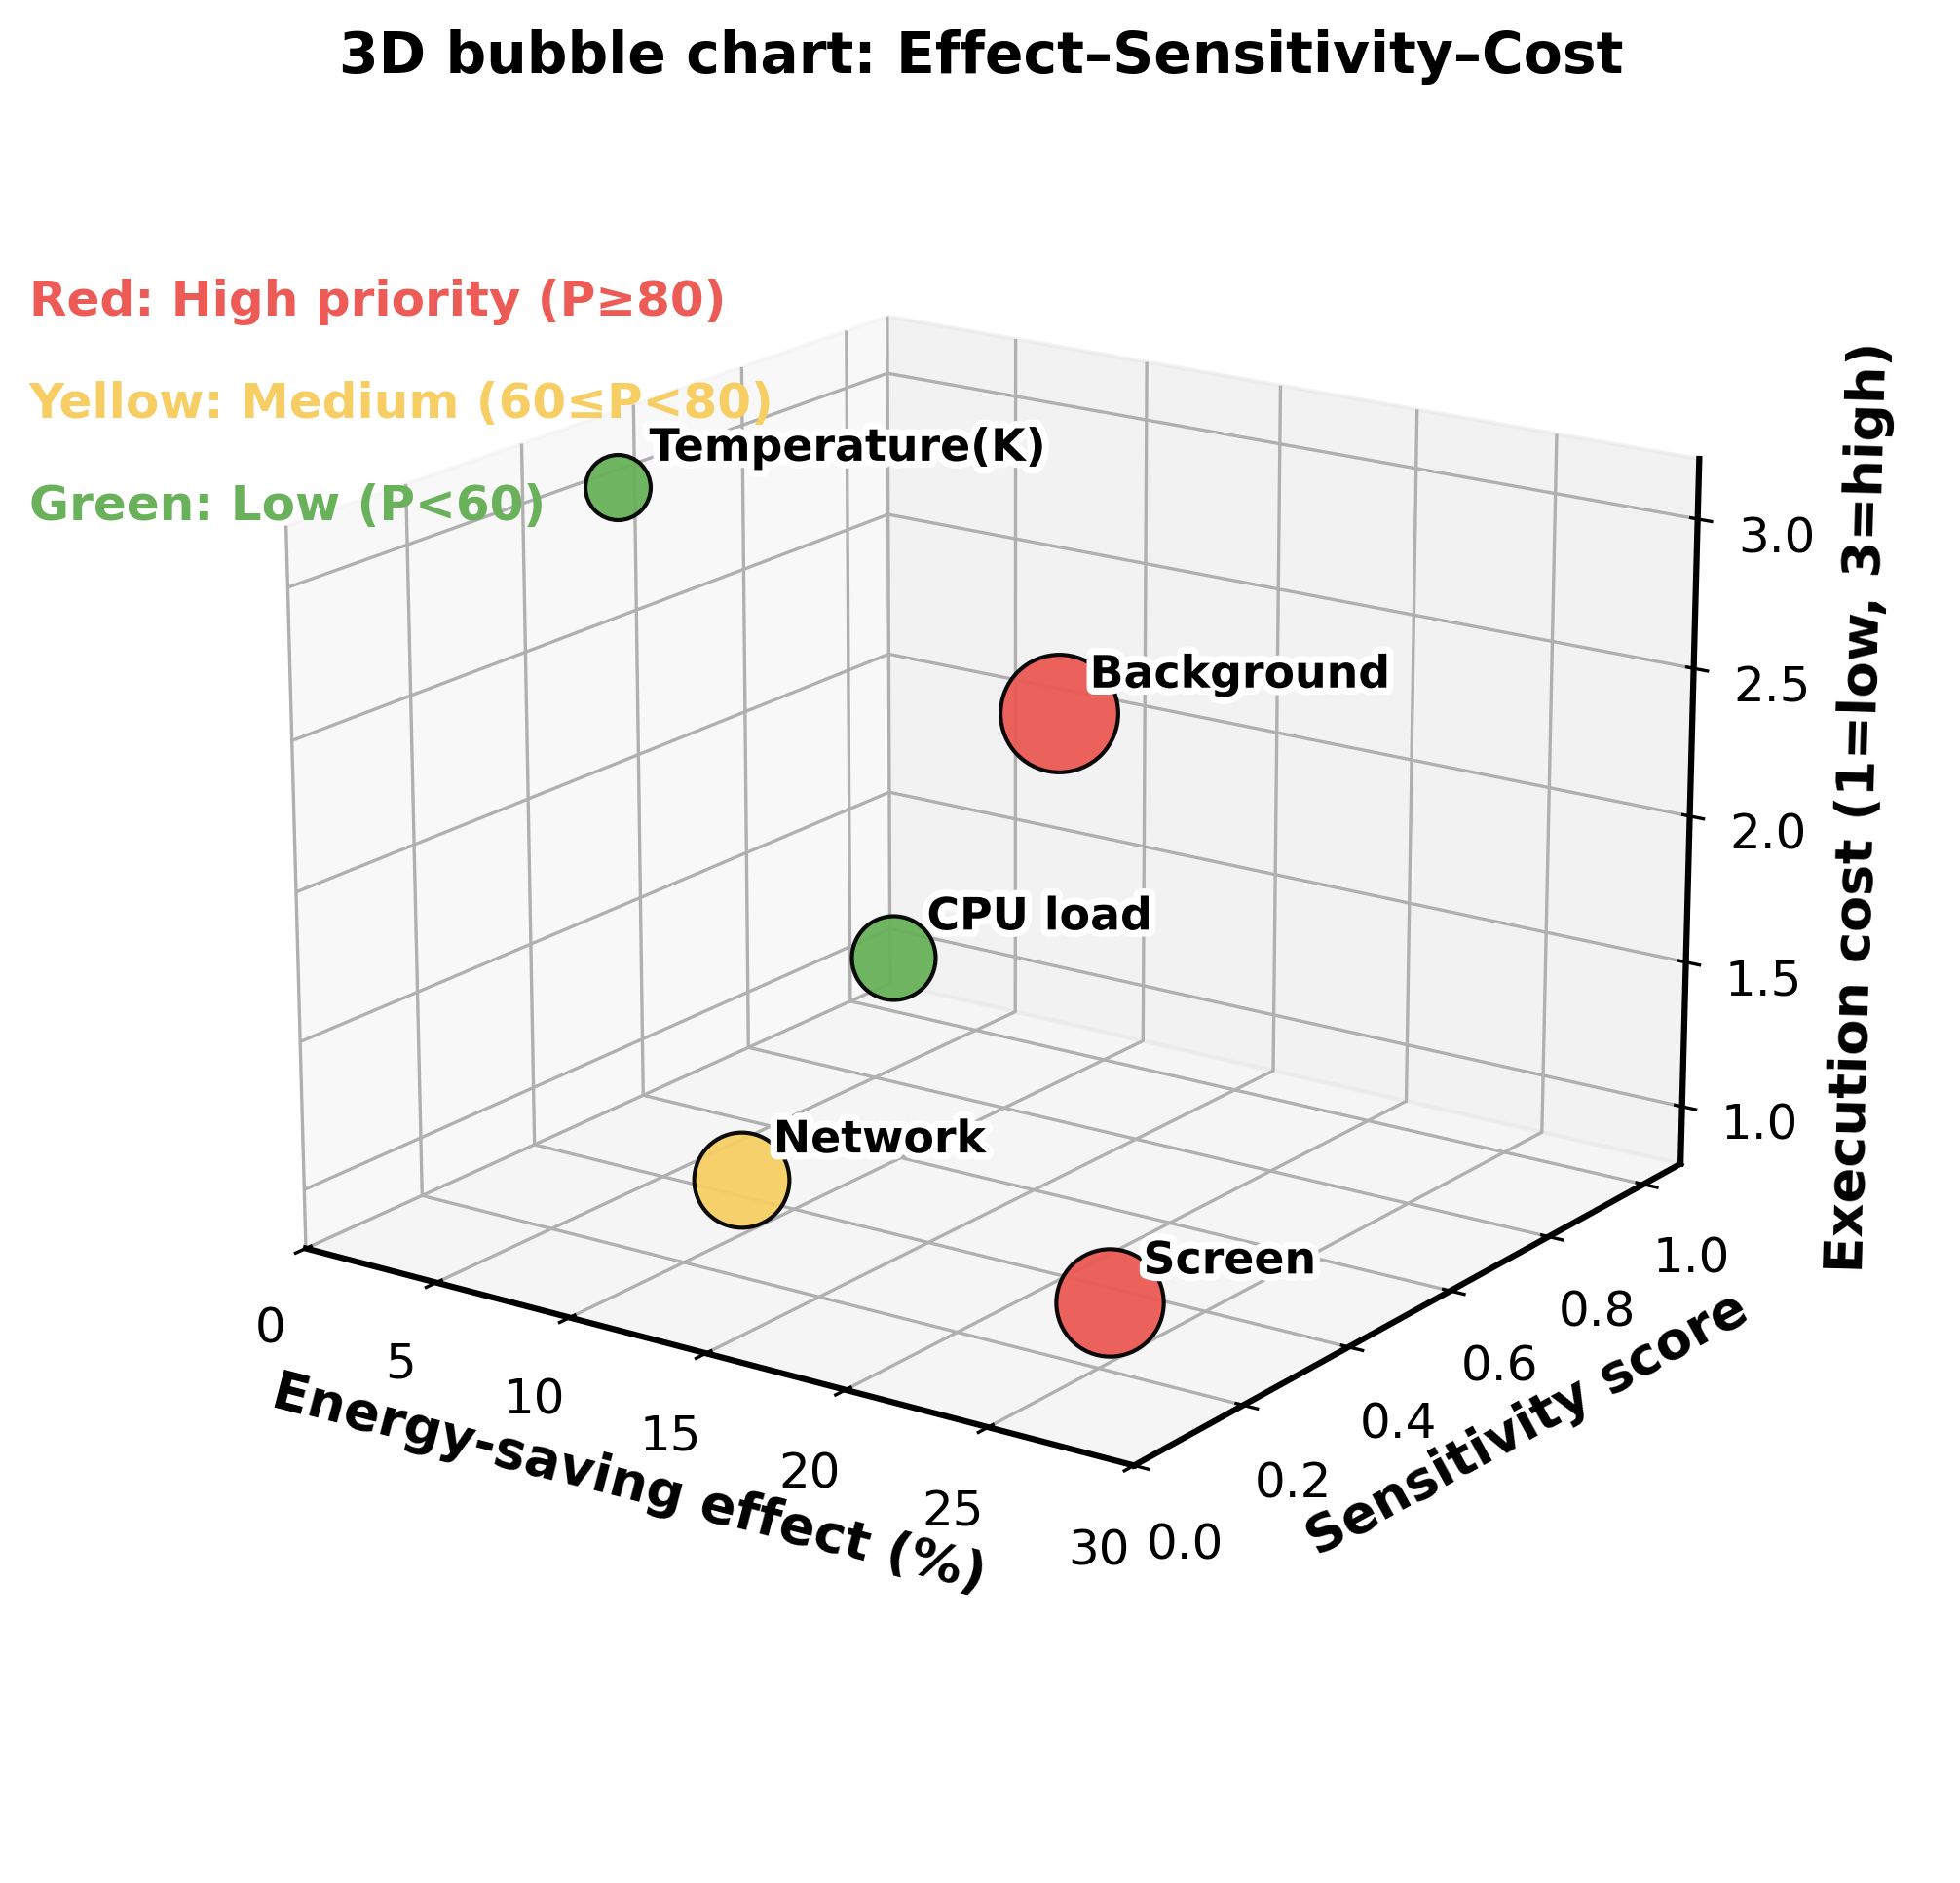
\includegraphics[width=\linewidth]{figures/task4_3D气泡图.jpg}
    \caption{\textbf{Multi-Dimensional Trade-off Analysis of Energy-Saving Strategies.} The spatial distribution visualizes the conflict between Sensitivity (Y), Energy-saving Potential (X), and Execution Cost (Z), with bubble colors indicating the final priority level.}
    \label{fig:3d_bubble}
  \end{minipage}\hfill
  \begin{minipage}{0.48\textwidth}
    \centering
    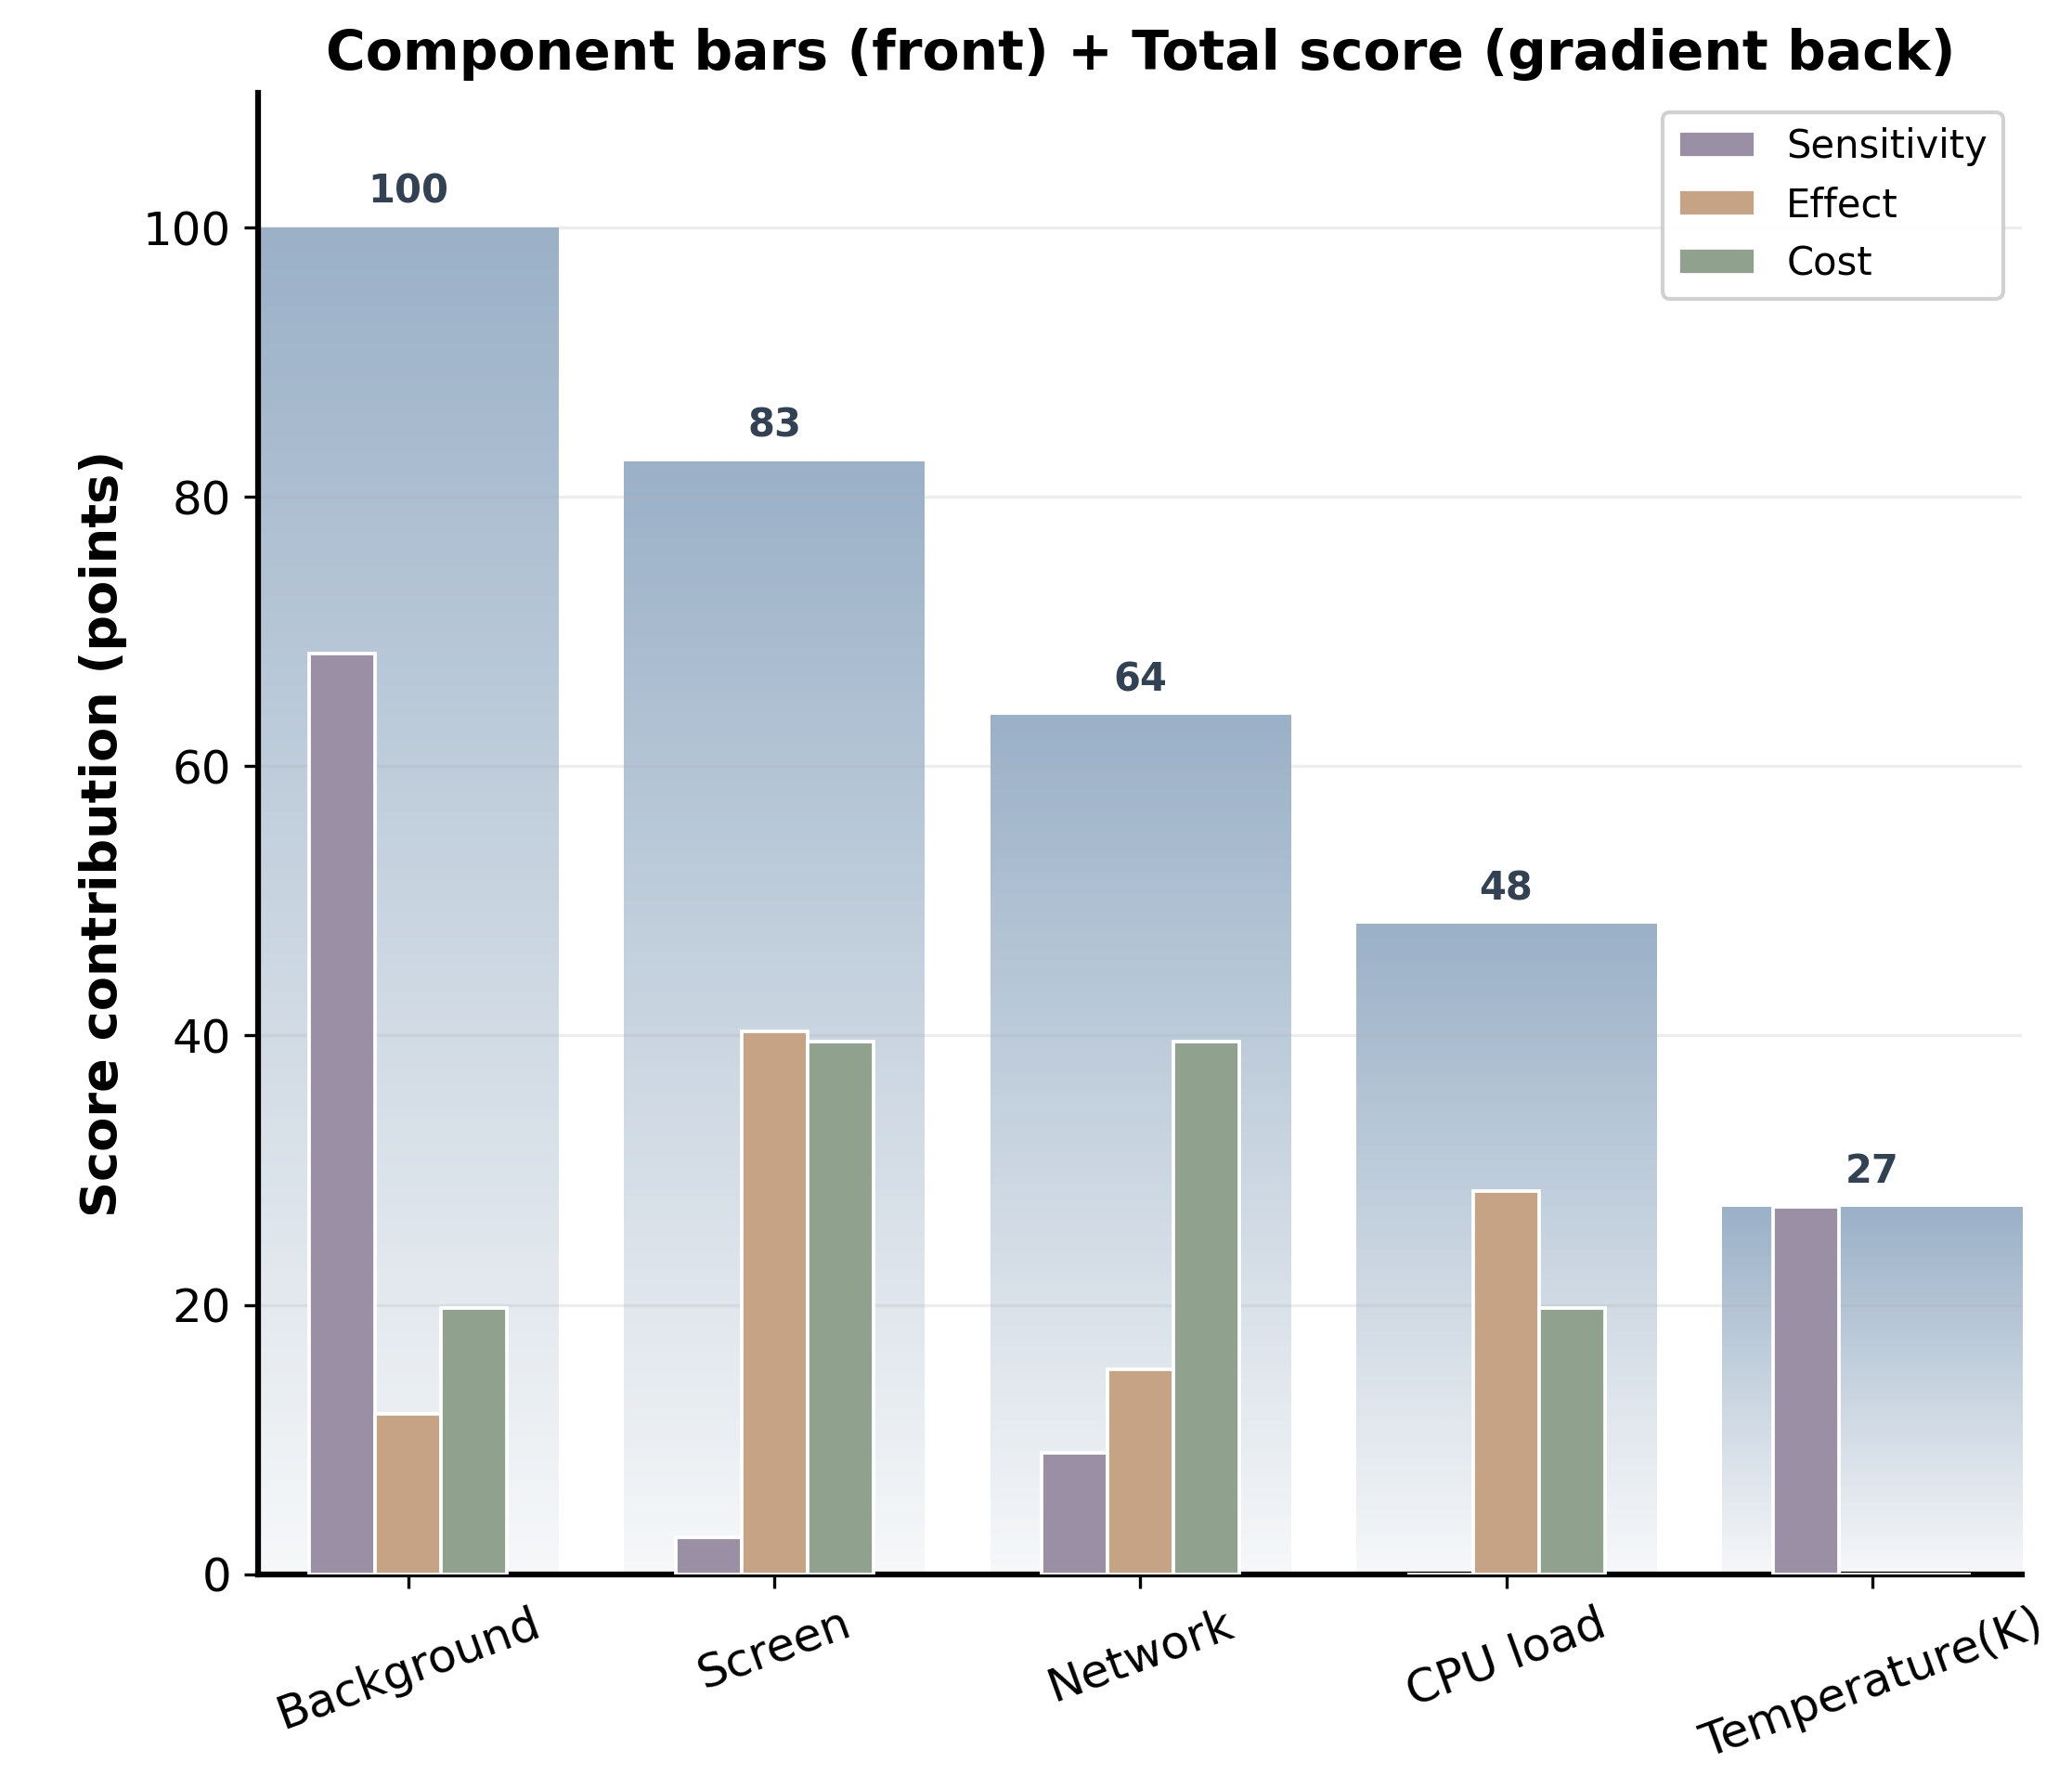
\includegraphics[width=\linewidth]{figures/task4_柱状堆叠图.jpg}
    \caption{\textbf{Decomposition of Comprehensive Priority Scores.} The chart ranks strategies by their total weighted score (gradient bars), while the inner stacked bars reveal the contribution of Sensitivity, Effect, and Cost to the final decision.}
    \label{fig:stacked_bar}
  \end{minipage}
\end{figure}

\subsection{Battery Aging Analysis}
To address the critical factor of long-term performance degradation, we integrate a \textbf{Battery Aging Model}. We define the \textbf{State of Health (SOH)} as the ratio of current maximum capacity to the nominal capacity:
\begin{equation}
\text{SOH}(t) = \frac{Q_{curr}(t)}{Q_{init}}
\end{equation}

where $Q_{init}$ is the nominal capacity and $Q_{curr}(t)$ is the current available capacity.

\paragraph{Dual-Factor Decay Mechanism}
We adopt a semi-empirical aging model that accounts for both calendar aging (time-dependent degradation) and cycle aging (active use).

\textbf{1. Calendar Aging ($\Delta Q_{cal}$):}
Calendar aging is driven by time and temperature, primarily due to the growth of the Solid Electrolyte Interphase (SEI) layer.
\begin{equation}
\Delta Q_{cal}(t, T, \SOC) = K_{cal} \cdot \exp\left(\frac{-E_{a,cal}}{R \cdot T(t)}\right) \cdot \SOC(t) \cdot t^{0.5}
\end{equation}
where $E_{a,cal}$ is the activation energy for calendar aging, and $t^{0.5}$ reflects the diffusion-limited nature of SEI growth.

\textbf{2. Cycle Aging ($\Delta Q_{cyc}$):}
Cycle aging results from the mechanical stress of lithium ion intercalation/de-intercalation during charging and discharging.
\begin{equation}
\Delta Q_{cyc}(N, T, I) = K_{cyc} \cdot \exp\left(\frac{-E_{a,cyc}}{R \cdot T_{avg}}\right) \cdot (I_{avg})^{\beta} \cdot \sqrt{Ah(N)}
\end{equation}
where $Ah(N)$ represents the total Ampere-hour throughput, and $\beta$ accounts for the impact of high C-rates.

\paragraph{Total Degradation \& Resistance Growth}
The total SOH is the combined effect of both aging mechanisms:
\begin{equation}
\text{SOH}_{total} = 1 - (\Delta Q_{cal} + \Delta Q_{cyc})
\end{equation}

Crucially, aging not only reduces capacity but also increases internal resistance, which we model as an exponential growth function:
\begin{equation}
R_{aged} = R_0 \cdot (1 + \gamma \cdot (1 - \text{SOH}_{total}))^\phi
\end{equation}
This coupled equation explains why aged batteries are more susceptible to sudden shutdowns in cold weather—the increased $R_{aged}$ amplifies the voltage drop ($V_{drop} = I \cdot R_{aged}$), triggering the cutoff voltage $V_{cutoff}$ earlier than fresh batteries.

\begin{figure}[H]
    \centering
    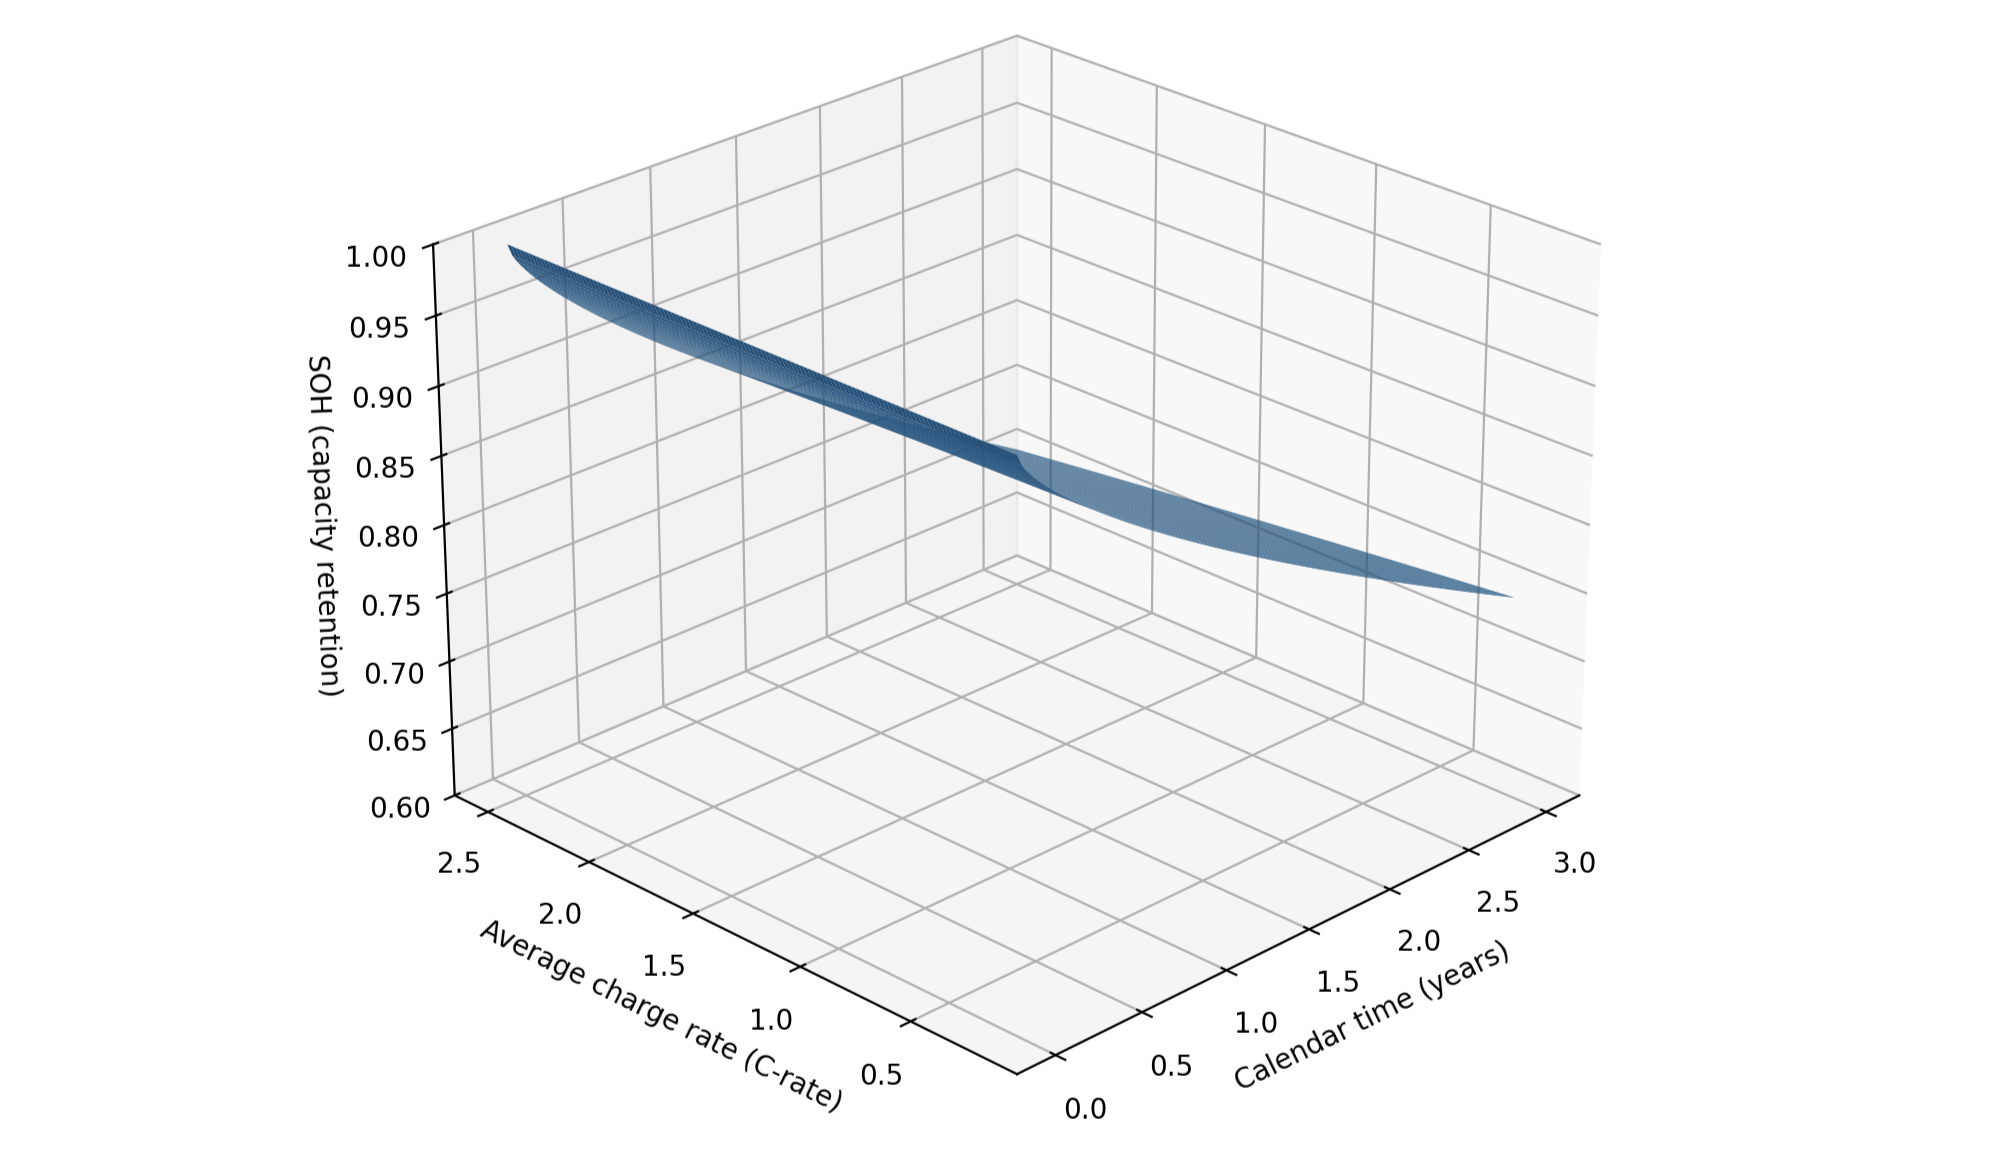
\includegraphics[width=0.8\textwidth]{figures/老化模型.png}
    \caption{\textbf{SOH Degradation Trajectory over Cycle Life.} The curve illustrates the non-linear decay of battery health. A 20\% drop in SOH (reaching EOL) results in a disproportionate $>25\%$ reduction in effective TTE under high-load conditions due to increased internal resistance.}
    \label{fig:aging_model}
\end{figure}

\subsection{Practical Recommendations}
\paragraph{User-Centric Behavioral Adjustments}
Our model identifies \textbf{Aggressive Background Management} as the single most effective intervention ($P_i=100$, High Priority). Since background processes have the highest sensitivity ($S_i=1.00$) and relatively low execution cost, users should strictly restrict background activity for non-essential apps. This yields the largest marginal gain in battery life. Secondly, \textbf{Smart Screen Dimming} ($P_i=82.6$) is critical. Although its sensitivity is lower, the sheer magnitude of its energy reduction potential ($E_i \approx 1.0$) makes it indispensable. We recommend users enable auto-brightness features that aggressively dim the screen in low-light environments.

\paragraph{System-Level Optimization (OS Developers)}
For operating systems, we propose a \textbf{"Thermal-Aware Adaptive Throttling"} mechanism. Our environmental impact analysis (Task 2) revealed that low temperatures significantly amplify internal resistance voltage drops. Therefore, the OS should dynamically cap peak CPU currents when the battery temperature drops below $10^\circ$C to prevent premature voltage cutoffs, effectively extending usable capacity in winter. Additionally, implementing an \textbf{"Eco-Mode"} that automatically freezes background threads when the screen is off directly targets the high-sensitivity background factor identified in our model.

\paragraph{Long-Term Health Maintenance}
Considering the non-linear decay of SOH shown in Figure \ref{fig:aging_model}, maintaining battery health is as crucial as daily energy saving. To mitigate \textbf{Calendar Aging}, users should avoid keeping the device at 100\% SOC for extended periods, as high SOC accelerates SEI layer growth. To reduce \textbf{Cycle Aging}, "shallow cycling" (charging before the battery drops below 20\%) is recommended to minimize mechanical stress on the electrodes.

\subsection{Future Outlook and Generalization}
A key strength of our \textbf{Component-Coupled Thevenin Framework} is its modularity. The core physics (Arrhenius Law, Thevenin ECM) and the Multi-Factor Power Model are universal. By simply recalibrating the component coefficients (e.g., $\beta$ for screen size, $\alpha$ for processor architecture) and the nominal capacity $\Qcap$, this framework can be generalized to other portable devices such as \textbf{tablets}, \textbf{smartwatches}, and even \textbf{electric vehicles (EVs)}, providing a unified solution for energy management across diverse platforms. Future work could integrate machine learning algorithms, such as LSTM networks, to predict user behavior patterns ($P_{load}(t)$) in real-time, further enhancing the accuracy of TTE predictions and the effectiveness of adaptive power management strategies.

% =========================================================
% 7. Strengths and Weaknesses
% =========================================================
\section{Strengths and Weaknesses}

\subsection{Strengths}
\begin{itemize}
    \item \textbf{Comprehensive Multi-Physics Coupling}: We successfully integrated electrochemical dynamics (Thevenin ECM), thermodynamics (Arrhenius Law), and user behavior. This holistic approach captures non-linear interactions better than isolated models.
    \item \textbf{Analytical Stability}: By deriving an exact quadratic solution for the power-voltage constraint, we eliminated the need for unstable iterative solvers. This ensures high computational efficiency and robustness.
    \item \textbf{Objective Decision Making}: Our recommendations rely on the CRITIC weighting method rather than subjective scoring. This ensures that our optimization strategies are strictly data-driven and unbiased.
    \item \textbf{Long-Term Perspective}: Unlike static models, our framework includes a semi-empirical aging model. This allows us to predict the State of Health (SOH) decay over time, offering valuable insights for the device's entire lifecycle.
\end{itemize}

\subsection{Weaknesses}
\begin{itemize}
    \item \textbf{Simplified Thermal Assumption}: We adopted a "Lumped Thermal Model" that assumes uniform temperature. This ignores local hotspots in the battery pack, which could accelerate aging faster than predicted.
    \item \textbf{Idealized User Behavior}: Our scenarios assume relatively stable loads. Real-world usage is highly stochastic (bursty). Consequently, our model might underestimate the stress caused by sudden peak currents.
    \item \textbf{Limited Granularity}: To ensure solvability, we aggregated peripheral components (like GPS and Sensors) into broader categories. This might reduce accuracy in specialized scenarios where these specific components dominate power consumption.
    \item \textbf{Idealized Health Assumption}: In Tasks 1 through 3, simulations were conducted under the assumption of a pristine battery ($SOH=1$) to mathematically isolate environmental factors from aging effects. Consequently, these baseline predictions represent a theoretical "upper bound" of performance and may not fully reflect the behavior of aged devices that suffer from capacity fade and increased internal resistance.
\end{itemize}

% =========================================================
% 8. Conclusion
% =========================================================
\section{Conclusion}
We have developed a comprehensive continuous-time model integrating component-level power dynamics and temperature-dependent electrochemical impedance. The analytical resolution of the power-voltage coupling ensures robust prediction capabilities across varying environmental conditions. Our sensitivity analysis highlights that while hardware components (Screen, CPU) draw significant power, environmental factors (Temperature) and software behavior (Background tasks) are critical, non-linear drivers of battery performance variability.

\begin{thebibliography}{99}
\bibitem{power_unpacked}
Carroll, A., \& Heiser, G. (2010). Power Efficiency Unpacked: Modeling Per-Component Power Consumption in Mobile Devices. \textit{USENIX}.

\bibitem{chen2006}
Chen, M., \& Rincon-Mora, G. A. (2006). Accurate electrical battery model capable of predicting runtime and IV performance. \textit{IEEE Transactions on energy conversion}, 21(2), 504-511.

\bibitem{zhang2025} 
Zhang, Q., Wang, F., \& Zhen, Q. (2025). Research on state of charge estimation of lithium battery based on adaptive forgetting factor recursive least squares and multi-innovation adaptive unscented Kalman filter. \textit{International Journal of Electrical and Energy Systems}. https://doi.org/10.1016/j.ijoes.2025.101103

\bibitem{wang2025} 
Wang, R., Liu, L., Zhang, H., et al. (2025). Collaborative estimation of lithium battery state of charge based on the BiLSTM-AUKF fusion model. \textit{Energies}, 18(21), 5624. https://doi.org/10.3390/en18215624

\bibitem{bressan2025} 
Bressan, M., Campagnoli, E., \& Giaretto, V. (2025). Experimental evidence on the effect of temperature on the performance of a lithium-ion battery. \textit{Batteries}, 11(12), 439. https://doi.org/10.3390/batteries11120439

\bibitem{aging_model}
Vetter, J., et al. (2005). Ageing mechanisms in lithium-ion batteries. \textit{Journal of Power Sources}, 147(1-2), 269-281.
\end{thebibliography}

\newpage
\vspace*{-1cm} % 向上调整距离
\section*{Memorandum}

\noindent
\begin{tabular}{ll}
\textbf{To:} & Smartphone Users \\
\textbf{From:} & MCM Team \#2622395 \\
\textbf{Date:} & February 2, 2026 \\
\textbf{Subject:} & Scientific Recommendations for Battery Care \\
\end{tabular}

\vspace{0.3cm}
\hrule
\vspace{0.4cm}

\textbf{Dear Smartphone User,}

In the digital age, battery anxiety is real. Sudden shutdowns in winter or rapid degradation are not accidents—they are physics. As the 2026 MCM research team, we built a \textbf{Thermal-Electrochemical Coupled Dynamics (TECD)} model to translate complex math into this practical "Battery Survival Guide."

\paragraph{1. Beware of the Cold (The Invisible Enemy)}
Our model reveals that low temperature is a silent killer. Below freezing, chemical reactions slow down, causing a massive spike in internal resistance. Launching a high-drain app (like a camera) creates a voltage drop that triggers an immediate shutdown, even with 30\% charge remaining. 
\textbf{Recommendation:} Warm your phone in your pocket before using it outdoors in freezing weather.

\paragraph{2. The 20-80\% Golden Rule}
Using our \textbf{Dual-Scale Adaptive Observer (DSAO)}, we found that keeping batteries at 100\% or 0\% accelerates the thickening of the internal SEI layer, permanently killing capacity.
\textbf{Recommendation:} Adopt "shallow cycling"—charge when you can to keep the level between 20\% and 80\%. Avoid high-load gaming while charging to prevent heat damage, which is the biggest accelerator of aging.

\paragraph{3. Smarter Future Systems}
We propose an \textbf{Adaptive Power Management Protocol (APMP)} for future OS designs. Phones should detect real-time internal resistance and throttle performance dynamically, ensuring stability for aging batteries rather than unexpected shutdowns.

Mathematical modeling serves to improve life. By adopting scientific habits, you save money and reduce electronic waste.

% --- 落款调整区域 ---
\vspace{2cm} % 增加垂直间距
\noindent \hfill % 填充空白，将内容推至右侧
\begin{minipage}[t]{3cm} % 创建一个宽5cm的文本框
    Sincerely yours,\\[0.5em] 
    Team \#2622395
\end{minipage}

\newpage
\section*{Report on Use of AI}

\begin{enumerate}
    \item \textbf{OpenAI ChatGPT (January 31, 2026 version, ChatGPT-5.2)}
    
    \textbf{Query1:} What is the typical battery capacity of smartphones on the market?
    
    \textbf{Output:} Most mainstream smartphones today have battery capacities in the 4,000–5,500 mAh range. Slimmer or smaller phones often sit around 3,500–4,500 mAh, while larger-screen and long-battery-life models are commonly about 5,000 mAh. A smaller number of phones that focus heavily on endurance can reach 6,000 mAh or more, but overall around 5,000 mAh is a very common “typical” capacity in recent years.

    \item \textbf{OpenAI ChatGPT (January 31, 2026 version, ChatGPT-5.2)}
    
    \textbf{Query2:} How does bootstrap quantify uncertainty?
    
    \textbf{Output:} Bootstrap quantifies uncertainty by repeatedly resampling your observed dataset with replacement to create many “new” pseudo-datasets, then re-running the same estimation procedure on each one (e.g., fitting your model and computing the parameter or prediction you care about). This produces an empirical distribution of the estimate across resamples. From that distribution, you can measure uncertainty using the standard deviation (as a standard error), percentile-based confidence intervals (e.g., the 2.5th–97.5th percentiles for a 95\% interval), and other summaries like bias or quantiles. In short, bootstrap turns the randomness of sampling into a concrete spread of results, so you can report how variable your parameters or predictions are without relying heavily on strict analytic assumptions.
\end{enumerate}

\end{document}